\chapter{
Introduction to GLMs and Bayesian Analysis
}
\markboth{Bayesian Analysis of GLMMS}{}
\label{chapt.glms}

\vspace{.3in}

%%%% STUFF TO DO
%%% 1. Prior lack of invariance to transformation stuff: Reference and Figure
%%% 4. reference for sampling from f() with bounded support
%%% 6. Check Bayesian p-value definition
%%% 8. spell check this document

%%% NEW STUFF TO DO
%%% add bugs model for BBS Poisson regression?
% XXX Should DIC/selection/FIT material go into Chapter 8? XXXXXXX

%%% some ref chapters need filling in; eg section 3.8; section 3.8.2
%%% Once Ch2 is ready, ask Richard to go over the sections on Poisson and Binommial GL(M)Ms to make sure there isn't too much redundancy between Ch2 and 3
%XXXX I commented out those sections that we agreed should be moved to Ch2, some stuff on Bayesian p value calculation

A major theme of this book is that spatial capture-recapture models
are, for the most part, just generalized linear models (GLMs) wherein
the covariate, distance between trap and home range center, is
partially or fully unobserved  -- and therefore regarded as
a random effect. Outside of capture-recapture, such models
are usually referred to as Generalized Linear Mixed Models (GLMMs)
and, therefore, SCR models can be thought of as a specialized type of
GLMM. Naturally then, we should consider analysis of these slightly
simpler models in order to gain some experience and, hopefully,
develop a better understanding of spatial capture-recapture models.

In this chapter, we consider classes of GLM models - Poisson and
binomial (i.e., logistic regression) GLMs - that will prove to be
enormously useful in the analysis of capture-recapture models of all
kinds. Many readers are likely familiar with these models already because
they are one of
the most useful models in all of ecology and, as
such, have received considerable attention in many introductory and
advanced texts. We focus on them here in order to introduce the
readers to the analysis of such models in {\bf R} and {\bf WinBUGS} or
{\bf JAGS},
which we will
translate directly to the analysis of SCR models in subsequent
chapters.

Bayesian analysis is convenient for analyzing GLMMs because it allows
us to work directly with the conditional model -- i.e., the model that
is conditional on the random effects, using computational methods
known as Markov chain Monte Carlo (MCMC). Learning how to do Bayesian
analysis of GLMs and GLMMs using the {\bf BUGS} language is, in part, the purpose
of this chapter. We focus here on the use of {\bf WinBUGS} because it
is the most popular ``{\bf BUGS} engine''. However, later in the book
we transition to another popular {\bf BUGS} engine known as {\bf
  JAGS} \citep{plummer:2009} which stands for {\it Just Another Gibbs
  Sampler}. For most of our purposes, the specification of models in
either platform is the same, but {\bf JAGS} is under active
development at the present time while {\bf WinBUGS} no longer is,
having transitioned to 
{\bf OpenBUGS} \citep{lunn_etal:2009} which is still in active
development.  
 While we use {\bf BUGS} of one sort or another to do the Bayesian
computations, we organize and summarize our data and execute {\bf
  WinBUGS} or {\bf JAGS} from within {\bf R} using the useful packages 
\mbox{\tt
  R2WinBUGS} \citep{sturtz_etal:2005}, \mbox{\tt R2jags} or \mbox{\tt rjags}.  \citet{kery:2010}, and
\citet{kery_schaub:2011} provide excellent and accessible introductions to the basics
of Bayesian analysis and GLMs using {\bf WinBUGS}.
We don't want to
be too redundant with those books and so we avoid a detailed
treatment of Bayesian methodology and software usage - instead just providing a cursory
overview so that we can move on and attack the problems we're most
interested in related to spatial capture-recapture.  In addition,
there are a number of texts that provide general introductions to
Bayesian analysis, MCMC, and their applications in ecology including
\citet{mccarthy:2007}, \citet{kery:2010}, \citet{link_barker:2010}, and
\citet{king_etal:2009}.


While this chapter is about Bayesian analysis of GLMMs, such models
are routinely analyzed using likelihood methods too, 
Later in
this book, we will use likelihood methods to analyze SCR models but,
for now, we concentrate on providing a basic introduction to Bayesian
analysis because that is the approach we will use in a majority of
cases in later chapters.

%Richard will move this section to previous chapter
% \section{ Notation}

% We will sometimes use conventional ``bracket notation'' \index{bracket
%   notation} to refer to
% probability distributions. If $y$ is a random variable then $[y]$
% indicates its distribution or its probability density/mass function
% (pdf, pmf) depending on context. If $x$ is another random variable
% then $[y|x]$ is the conditional distribution of $y$ given $x$, and
% $[y,x]$ is the joint distribution of $y$ and $x$. To differentiate
% specific distributions in some contexts we might label them $g(y)$,
% $g(y|\theta)$, $f(x)$, or similar. We will also write $y \sim
% \mbox{Normal}(\mu,\sigma^{2})$ to indicate that $y$ ``is distributed as'' a normal
% random variable with parameters $\mu$ and $\sigma^{2}$. The expected value
% or mean of a random variable is $E[y] = \mu$ ,and $Var[y] = \sigma^{2}$ is
% the variance of $y$.   To indicate specific observations we'll use an
% index such as ``$i$''. So, $y_{i}$ for $i=1,2,\ldots,n$ indicates
% observations for $n$ individuals. Finally, we write $\Pr(y)$ to indicate specific probabilities, i.e., of events ``$y$'' or similar.


% To illustrate these concepts and notation, suppose $z$ is a binary
% outcome (e.g., species occurrence) and we might assume the model: $z
% \sim \mbox{Bern}(p)$ for observations.  Under this model $\Pr(z=1) =
% \psi$, which is also the expected value $E[z] = \psi$. The variance is
% $Var[z] = \psi*(1-\psi)$ and the probability mass function (pmf) is $[z]
% = \psi^{z} (1-\psi)^{1-z}$. Sometimes we write $[z|\psi]$ when it is
% important to emphasize the conditional dependence of $z$ on $\psi$. As
% another example, suppose $y$ is a random variable denoting whether or
% not a species is detected if an occupied site is surveyed. In this
% case it might be natural to express the pmf of the observations $y$
% {\it conditional} on $z$. That is, $[y|z]$. In this case, $[y|z=1]$ is
% the conditional pmf of $y$ given that a site is occupied, and it is
% natural to assume that $[y|z=1] = \mbox{Bern}(p)$ where $p$ is the
% ``detection probability'' - the probability that we detect the
% species, given that it is present. The model for the observations $y$
% is completely specified once we describe the other conditional pmf
% $[y|z=0]$. For this conditional distribution it is sometimes
% reasonable to assume $\Pr(y=1|z=0) = 0$ (\citet{mackenzie_etal:2002};
% see also \citet{royle_link:2006}). That is, if the species is absent,
% the probability of detection is 0. This implies that
% $\Pr(y=0|z=0)=1$. To allow for situations in which the true state $z$
% is unobserved, we  assume that $[z]$ is Bernoulli with parameter
% $\psi$.  In this case, the marginal distribution of $y$ is
% \[
%  [y] = [y|z=1]Pr(z=1) + [y|z=0]Pr(z=0)
% \]
% because $[y|z=0]$ is a point mass at $y=0$, by assumption, the marginal
% probability that $y=1$ is
% \[
% \Pr(y=1) = p \psi
% \]
% and the marginal probability that $y=0$ is
% \[
% \Pr(y=0) = (1-p)*\psi + (1-\psi)
% \]
%END of section Richard will move to previous chapter

\section{
GLMs and GLMMs}
\label{glms.sec.glmms}
We have asserted already that SCR models work out most of the time to
be variations of GLMs and GLMMs. You might therefore ask: What
are GLMs and GLMMs, anyhow?   These models are covered extensively in
many very good applied statistics books and we refer the reader
elsewhere for a detailed introduction.  The
classical reference for GLMs is \citet{nelder_wedderburn:1972} and
also \citet{mccullagh_nelder:1989}. In addition, we think \citet{kery:2010},
\citet{kery_schaub:2011}, and \citet{zuur_etal:2009} are all
accessible treatments of considerable merit. 
Here, we'll give the 1
minute
treatment of GLMMs, not trying to be complete but rather only
to preserve a coherent organization to the book.


The generalized linear model (GLM) is an extension of standard linear
models by allowing the response
variable to have some distribution from the exponential family of
distributions (i.e., not just normal). This includes the normal
distribution but also others such as the Poisson, binomial,
gamma, exponential, and many more. In addition, GLMS allow the
response variable to be related to the predictor variables (i.e.,
covariates) using a link function, which is usually nonlinear.  
%Finally, GLMs typically
% accommodate a relationship between the mean and variance.
% The GLM consists of three components:
% \begin{itemize}
% \item[1.] A probability distribution for the dependent variable $y$,
% from the exponential family of probability distributions.
%\item[2.] A ``linear predictor'' $\eta = {\bf x}'{\bm \beta}$  .
% \item[2.] A ``linear predictor'' $\eta = \beta_0 + x \beta_1$, where $x$ is the predictor variable.
% \item[3.] A link function $g$ that relates $E[y]$ to the linear predictor, $E[y] = \mu = g^{-1}(\eta)$. Therefore $g(E[y]) = \eta$.
% \end{itemize}
% XXXX ISNT THIS REDUNDANT? XXXXXXXXX
% The dependent variable $y$ is assumed to be an outcome from a
% distribution of the exponential family. The mean of the distribution of $y$ is assumed to depend on predictor variables $x$ according to
% \[
%  %g(E[y]) = {\bf x}'{\bm \beta}
%  g(E[y]) =\beta_0 + x \beta_1
% \]
% where $E[y]$ is the expected value of $y$, and ${\bf x}'{\bm \beta}$
% is termed the {\it linear predictor}, i.e., a linear function of the
% predictor variables ${\bf x}$ with unknown parameters ${\bm \beta}$ to be
% estimated.  
% The function $g$ is the link function. In standard GLMs,
% the variance of $y$ is a function $V$ of the mean of $y$: $Var(y) =
% V(\mu)$ (see below for examples).
% XXXXXXXXXXXXXXXXXXXXXXXXXXXXXXXXXXXXX SEEMS REDUNDANT UP TO HERE XXXXXXXXXXXXXXXX
The GLM consists of three components:
\begin{itemize}
\item[1.] A probability distribution for the dependent variable $y$,
from the exponential family of probability distributions.
\item[2.] A ``linear predictor'' $\eta = \beta_0 + x \beta_1$, where
  $x$ is a predictor variable (i.e., a covariate).
\item[3.] A link function $g$ that relates the expected value of $y$, $\mathbb{E}(y)$, to the linear predictor, $\mathbb{E}(y) = \mu = g^{-1}(\eta)$. Therefore $g(\mathbb{E}(y)) = \eta = \beta_0 + x \beta_1$ .
\end{itemize}
A key aspect of GLMs is that 
$g(\mathbb{E}(y))$ is assumed to be a linear function of the
predictor variable(s), here $x$, with unknown parameters, here $\beta_0$ and $\beta_1$, to be
estimated. In standard GLMs,
the variance of $y$ is a function $V$ of the mean of $y$: $\mbox{Var}(y) =
V(\mu)$ (see below for examples).
As an example, a Poisson GLM posits that $y \sim \mbox{Poisson}(\lambda)$ with $\mathbb{E}[y]
=\lambda$ and usually the model for the mean is specified using the
{\it log link function} by
\[
{\text log}(\lambda_{i}) = \beta_0 + \beta_{1}  x_{i}
\]
The variance function is $\mbox{V}(y_{i}) = \lambda_{i}$.  

To see how a Poisson GLM works, use the {\bf R} code below to simulate
some data and then estimate the parameters:
\begin{verbatim}
set.seed(13)
n=100 #set sample size
beta0<- -2 # set intercept term
beta1<- 1.5 #set coefficient
x<-rnorm(n, 0,1) #generate a predictor variable, x
linpred<- beta0 + beta1*x # calculate the linear predictor of E[y]
y<-rpois(n, exp(linpred)) # generate observations, y, from above model
\end{verbatim} 
The {\bf R} function {\tt glm()} fits a GLM to the data we just
generated and returns estimates of $\beta_0$ and $\beta_1$, which we
see are fairly close to the data generating values above:
\begin{verbatim}
glm(y~1+x, family='poisson') #fit model
\end{verbatim}
This produces the output:
\begin{verbatim}
Call:  glm(formula = y ~ 1 + x, family = "poisson")

Coefficients:
(Intercept)            x  
     -2.007        1.446  

[... some output deleted ...]
\end{verbatim}

The
binomial GLM posits that $y_{i} \sim \mbox{Binomial}(K,p)$ where $K$
is the fixed sample size parameter and $\mathbb{E}(y_{i}) = K*p_{i}$. Usually
the model for the mean is specified using the {\it logit link
  function} according to
\[
 \text {logit}(p_{i}) = \beta_{0} + \beta_{1}  x_{i}
\]
Where $\text {logit}(u) = \text {log}(u/(1-u))$.  The inverse-logit function,
consequently, is $\text {logit}^{-1}(u) =
\text {exp}(u)/(1+\text {exp}(u))$.

A GLMM is the extension of GLMs to accommodate ``random
effects''. Often this involves adding a normal random effect to the
linear predictor, and so a simple example is:
\[
 \log(\lambda_{i}) = \alpha_{i} + \beta_{1} x_{i}
\]
where
\[
 \alpha_{i} \sim \mbox{Normal}(\mu,\sigma^{2})
\]
Many other probability distributions and formulations of the linear
predictor might be considered.  GLMMs are enormously useful in
ecological modeling applications for modeling variation due to 
subjects, observers, spatial
or temporal stratification, clustering, and dependence that arises
from any kind of group structure.

%It is not widely appreicated that
%the link function and
%distribution of the random effect interact directly to affect the
%implied probability distribution of the linear predictor. For the
%Poisson case just considered, $\lambda_{i}$ has a log-normal
%distribution. However, if we set $\lambda_{i} = \alpha_{i}exp(\beta*x_{i})$
%where $\alpha_{i}$ has a Gamma distribution, then $\lambda_{i}$ has
%similarly a gamma distribution with modified scale parameter.  These
%different model assumptions are seldom evaluated formally in practice
%although in many practical situations (in ecology), they imply
%specific things about the ecological process being studied
%(e.g., see \citet{royle_dorazio:2008} section XYZ on occupancy
%logit/cloglog etc..).



\section{Bayesian Analysis}

Bayesian analysis is unfamiliar to many ecological researchers because
older cohorts of ecologists were largely educated in the classical
statistical paradigm of frequentist inference. But advances in
technology and increasing exposure to the benefits of Bayesian analysis
are fast making Bayesians out of people or at least making Bayesian
analysis an acceptable, general alternative to classical, frequentist
inference.

Conceptually, the main thing about Bayesian inference is that it uses
probability directly to characterize uncertainty about things we don't
know.  ``Things'', in this case, are parameters of models and, just as
it is natural to characterize uncertain outcomes of stochastic
processes using probability, it seems natural also to characterize
information about unknown parameters using probability. At least
this seems natural to us and, we think, most ecologists either
explicitly adopt that view or tend to fall into that point of view
naturally.  Conversely, frequentists use probability in many different
ways, but never to characterize uncertainty about
parameters\footnote{To hear this will be shocking to some readers
  perhaps.}. Instead, frequentists use probability to characterize the
behavior of {\it procedures} such as estimators or confidence
intervals (see below). It is surprising that people readily
adopt a philosophy of statistical inference in which the things you
don't know (i.e., parameters) should {\it not} be regarded as random
variables, so that, as a consequence, one cannot use probability to
characterize one's state of knowledge about them.


\subsection{Bayes' Rule}

As its name suggests, Bayesian analysis makes use of Bayes' rule in
order to make direct probability statements about model
parameters. Given two random variables $z$ and $y$, Bayes' rule relates
the two conditional probability distributions $[z|y]$ and $[y|z]$ by
the relationship:
\begin{equation}
[z|y] = [y|z][z]/[y]
\label{glms.eq.bayes}
\end{equation}
Bayes' rule itself is a mathematical fact and there is no debate in
the statistical community as to its validity and relevance to many
problems. Generally speaking, these distributions are characterized as
follows: $[y|z]$ is the conditional probability distribution of $y$
{\it given} $z$, $[z]$ is the marginal distribution of $z$ and $[y]$
is the marginal distribution of $y$. In the context of Bayesian
inference we usually associate specific meanings in which $[y|z]$ is
thought of as ``the likelihood'', $[z]$ as the ``prior'' and so on. We
leave this for later because here the focus is on this expression of
Bayes' rule as a basic fact of probability.

As an example of a simple application of Bayes' rule,
consider the problem of determining species presence at a sample
location based on imperfect survey information. Let $z$ be a binary
random variable that denotes species presence $(z=1)$ or absence
$(z=0)$, let $\Pr(z=1) = \psi$ where $\psi$ is usually called
occurrence probability, ``occupancy'' \citep{mackenzie_etal:2002} or ``prevalence''.
Let $y$ be the {\it observed} presence
($y=1$) or absence ($y=0$) (or, strictly speaking, detection and non-detection), and let $p$ be the probability that a
species is detected in a single survey at a site given that it is
present. Thus, $\Pr(y=1|z=1)=p$. The interpretation of this is that,
if the species is present, we will only observe it with
probability $p$. In addition, we assume here that $\Pr(y=1|z=0) =
0$. That is, the species cannot be detected if it is not present which
is a conventional view adopted in most biological sampling problems (but
see \citet{royle_link:2006}).
If we survey a site $K$ times but never detect the species,
then this clearly does not imply that the species is not present
($z=0$) at this site (we could just fail to observe it every single time). Rather, our degree of belief in $z=0$ should be
made with a probabilistic statement,
$\Pr(z=1|y_1=0,\ldots,y_{K}=0)$. If the $K$ surveys are independent so
that we might regard $y_{k}$ as $iid$ Bernoulli trials, then the total
number of detections, say $y$, is Binomial with probability $p$, and
we can use Bayes' rule to compute the probability that the species is present
given that it is not detected in $K$ samples. In words, the expression
we seek is:
\[
\Pr(\mbox{present} | \mbox{not detected}) = \frac{\Pr(\mbox{not detected} |
  \mbox{present})\Pr(\mbox{present})}{\Pr(\mbox{detected})}
\]
Mathematically, this is
\begin{eqnarray*}
\Pr(z=1|y=0) &= &\frac{\Pr(y=0|z=1)\Pr(z=1)}{\Pr(y=0) } \\
             &= & \frac{(1-p)^{K} \psi}{ (1-p)^K \psi + (1-\psi) }.
\end{eqnarray*}
To apply this,
suppose that $K=2$ surveys are done at a wetland for a species of
frog, and the species is not detected there. Suppose further that $\psi
= 0.8$ and $p = 0.5$ are obtained from a prior study.  Then the
probability that the species is present at this site is
$(1-0.5)^2 \times 0.8/((1-0.5)^2 \times 0.8 + (1-0.8)) = 0.5$. 
That is, there seems to be about a
50/50 chance that the site is occupied despite the fact that the
species wasn't observed there.

In summary, Bayes' rule provides a simple linkage between the
conditional probabilities $[y|z]$ and $[z|y]$, which is useful whenever
we need to deduce one from the other.

\subsection{Bayesian Inference}

Bayes' rule as a basic fact of probability is not disputed.
What is controversial to some is the scope and manner in which Bayes'
rule is applied by Bayesian analysts. Bayesian analysts assert that
Bayes' rule is relevant, in general, to all statistical problems by
regarding all unknown quantities of a model as realizations of random
variables - this includes data, latent variables, and also
parameters. Classical (non-Bayesian) analysts sometimes object to
regarding parameters as outcomes of random variables. Classically,
parameters are thought of as ``fixed but unknown'' (using the
terminology of classical statistics).
Indeed, a common misunderstanding on the distinction between Bayesian and
frequentist inference goes something like this ``in frequentist
inference parameters are fixed but unknown but in a Bayesian analysis
parameters are random.'' At best this is a sad caricature of the
distinction and at worst it is downright wrong. 
In Bayesian analysis the
parameters are also unknown and, in fact, there is a single data-generating
value of each parameter, and so they are also fixed.
The difference is that the fixed
but unknown values are  regarded as having been generated from some
probability distribution. Specification of that probability
distribution is necessary to carryout Bayesian analysis, but it is not
required in classical frequentist inference.


To see the general relevance of Bayes' rule in the context of
statistical inference, let $y$ denote observations - i.e., data -
and let $[y|\theta]$ be the observation model (often colloquially
referred to as the ``likelihood'').  Suppose $\theta$ 
is a parameter of
interest having (prior) probability distribution $[\theta]$. These are
combined to obtain the posterior distribution using Bayes' rule, which
is:
\[
 [\theta|y]= [y|\theta][\theta]/[y]
\]
Asserting the general relevance of Bayes' rule to all statistical
problems, we can conclude that the two main features of Bayesian
inference are that: (1) parameters, $\theta$, are regarded as realizations of
a random variable and, as a result, (2) inference is based on the
probability distribution of the parameters given the data,
$[\theta|y]$,
which is
called the posterior distribution. This is the result of using Bayes'
rule to combine the ``likelihood'' and the prior distribution.  The
key concept is regarding parameters as realizations of a random
variable because, once you admit this conceptual view, this leads
directly to the posterior distribution, a very natural quantity upon
which to base inference about things we don't know -  including
parameters of statistical models.  In particular, $[\theta|y]$ is a
probability distribution for $\theta$ and therefore we can make direct
probability statements to characterize uncertainty about
$\theta$.

The denominator of our invocation of Bayes' rule, $[y]$,
is the marginal distribution of the data $y$.  We note without further
remark right now that, in many practical problems, this can be an
enormous pain to compute. The main reason that the Bayesian paradigm
has become so popular in the last 20 years or so is because methods
have been developed
for characterizing the posterior distribution that do not
require that we possess a mathematical understanding of $[y]$. This means,
we never have to compute it or know what it looks like, or know
anything specific about it.

%A Bayesian
%assumes, just like a frequentist, that there was a single
%data-generating value of that parameter - a fixed, and unknown value
%that produced the given data set.
%The distinction between Bayesian and frequentist approaches is that
%Bayesians regard the parameter as a random variable, and its value as
%the outcome of a random variable, on par with the observations. 


While we can understand the conceptual basis of Bayesian inference
merely by understanding Bayes' rule -- that's really all there is to it
-- it is not so easy to understand the basis of classical
frequentist inference. 
% which is mostly like
% \footnote{as characterized by Christopher A. Sims, winner of the 
% Sveriges Riksbank Prize in Economic Sciences in Memory of Alfred Nobel
% in his
% Hotelling Lecture 6/29/2007 at Duke University - 
% \url{http://sims.princeton.edu/yftp/EmetSoc607/AppliedBayes.pdf}:
% ``Bayesian inference is a way of thinking,
% not a basket of 'Methods'''} a ``basket of
% methods'' with little coherent organization. 
What is mostly coherent
in frequentist inference is the manner in which items are evaluated -- the performance of a given procedure is
evaluated by ``averaging over'' hypothetical realizations of $y$,
regarding the {\it estimator} as a random variable. For example, if
$\hat{\theta}$ is an estimator of $\theta$ then the frequentist is
interested in $E_{y}[\hat{\theta}|y]$ which is used to characterize
bias. If the expected value of $\hat{\theta}$, when averaged over
realizations of $y$, is equal to $\theta$, then $\hat{\theta}$ is
unbiased.

The view of parameters as being random variables 
allows Bayesians to use probability to make direct probability
statements about parameters. Frequentist inference procedures do not
permit direct probability statements to be made about parameter
values.
Instead, 
the view of parameters as fixed constants and estimators as random variables
leads to interpretations that are not so straightforward. For
example confidence intervals having the interpretation ``95\%
probability that the interval contains the true value" and p-values
being "the probability of observing an outcome as extreme or more than
the one observed.'' These are far from intuitive interpretations to
most people.  Moreover, this is conceptually problematic to some
because the hypothetical realizations that characterize the
performance of our procedure we will never get to observe.

While we do tend to favor Bayesian inference for the conceptual
simplicity (parameters are random, posterior inference), we mostly
advocate for a pragmatic non-partisan approach to inference because,
frankly, some of the frequentist methods are actually very
convenient in certain situations as we will see in later chapters.


\subsection{Prior distributions}
%add paper richard mentioned in the meeting...

The prior distribution $[\theta]$ is an important feature of Bayesian
inference. As a conceptual matter,
the prior distribution characterizes ``prior beliefs'' or ``prior
information'' about a parameter. Indeed,
an oft-touted benefit of Bayesian analysis is the ease with which
prior information can be included in an analysis. 
However, more commonly, the prior is chosen to
express a lack of prior information, even if previous studies have
been done and even if the investigator does in fact know quite a bit
about a parameter.
This is because
the manner in which prior information is embodied in a prior (and the
amount of information) is
usually very subjective and thus the result can wind up being very
contentious, e.g., different investigators might report different
results based on subjective assessments of prior information. Thus it is usually
better to ``let the data speak'' and use priors that reflect absence
of information beyond the data set being analyzed. An example for an uninformative prior is a $\mbox{Uniform}(0,1)$ for a probability, or a \mbox{Uniform}(-$\infty$, $\infty$) (also called a ``flat'' or ``improper'' prior) for an unbounded continuous parameter. Alternatively, people use ``diffuse priors''; these contain some information, but (ideally) not enough to actually influence the posterior. An example for a diffuse prior could be a Normal distribution with a large standard deviation.

But still the need occasionally arises to embody prior information or
beliefs about a parameter formally into the estimation scheme.
 In SCR models we often have a parameter that is closely linked
to ``home range size'' and thus auxiliary information on the home
range size of a species can be used as prior information, which may improve parameter estimation (e.g., see
\citet{chandler_royle:2012} ; also Chapt. \ref{chapt.scr-unmarked}).

Other times the situation arises where a prior can inadvertently impose
substantial information on a parameter, and that is not desirable.
For example, we use data augmentation
to deal with the fact that $N$ is an unknown parameter
 \citep{royle_etal:2007} which is equivalent to imposing a $\mbox{Binomial}(M,\psi)$
 prior on $N$ for some integer $M$. One has to take care to make sure
 that $M$ is sufficiently large so as to not affect the posterior
 distribution on $N$ (see Fig. \ref{mcmc.fig.timeseries2}, and also
 \citet[][Ch. 5]{kery_schaub:2011}).
Another situation that we have
 to be careful of is that
prior 
distributions are {\it not} invariant to transformation of the
parameter,
and therefore neither are posterior distributions
\citep[][sec. 6.2.1]{link_barker:2010}. Thus, a prior that is ostensibly
non-informative on one scale, may be very informative on another
scale. 
For example, if we have a flat prior on $\mbox{logit}(p)$ for some probability
parameter $p$, this is very different from having a 
$\mbox{Uniform}(0,1)$ prior 
on $p$. We show an example where this makes a difference in
Chapt. \ref{chapt.scr0}. Nonetheless, it is always possible to assess
the influence of prior choice, and it is often the case (with
sufficient data and a structurally identifiable model) that the
influence of priors is neglibible. 

\subsection{Posterior Inference}

In Bayesian inference, we are not focusing on estimating a single
point or interval but rather on characterizing a whole distribution --
the posterior distribution -- from which one can report any summary of
interest. A point estimate might be the posterior mean, median, mode,
etc..  In many applications in this book, we will compute 95\%
Bayesian confidence intervals using the 2.5\% and 97.5\% quantiles of the
posterior distribution. For such intervals, it is correct to say
$\Pr(L < \theta < U) = 0.95$. That is, ``the probability that $\theta$
is between $L$ and $U$ is $0.95$". 

As an
example, suppose we conducted a Bayesian analysis to estimate
detection probability ($p$) of some species at a study site, and we
obtained a posterior distribution of beta(20,10) for the parameter
$p$. The following {\bf R} commands demonstrate how we make inferences based
upon summaries of the posterior distribution:
\begin{verbatim}
> post.median <- qbeta(0.5, 20, 10)
[1] 0.6704151
> post.95ci <- qbeta(c(0.025, 0.975), 20, 10)
[1] 0.4916766 0.8206164
\end{verbatim}
Thus, we can state that there is a 95\% probability that $\theta$ lies
between 0.49 and 0.82. Fig. \ref{densityvsdetection.fig} shows the
posterior along with the summary statistics.

\begin{figure}
\begin{center}
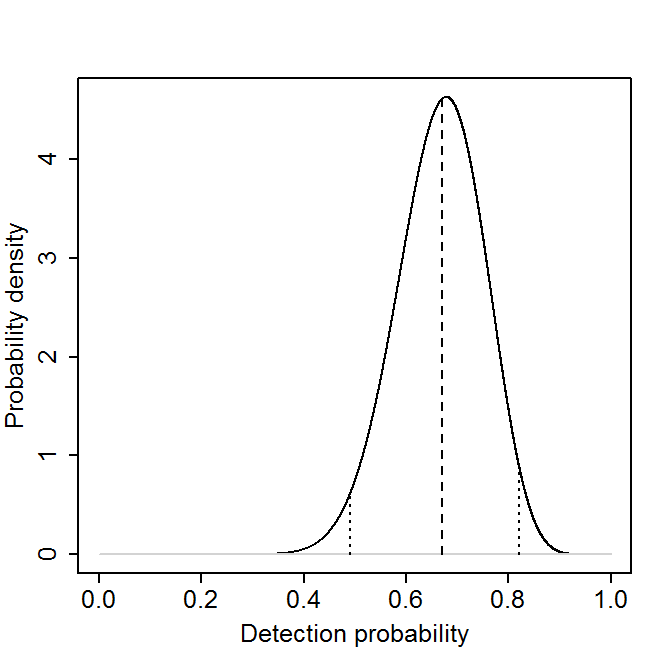
\includegraphics[height=2.5in]{Ch2-Bayes/figs/densityvsdetection}
%get figure file from Ch7 folder
\end{center}
\caption{Probability density plot of a hypothetical
 posterior distribution of beta(20,10); dashed lines 
 indicate mean and upper and lower 95\% interval}
\label{densityvsdetection.fig}
\end{figure}

It is not a subtle thing that this
cannot be said using frequentist methods, although people tend to say
it anyway and not really understand why it is wrong or even that it is
wrong. This is  because %actually a failing of frequentist ideas and the
%inability of frequentists to get
frequentists have not been successful in convincing people to
over-ride their natural inclination on how to use probability.  As a
frequentist, you simply cannot use probability in the manner that you
would like to.


% As a conceptual matter, Bayesian inference based on the posterior
% allows us 
%  to make an inference conditional on the data that we
% actually observed, i.e., what we actually know.  To us, this seems
% logical - to condition on what we know. Conversely, frequentist
% inference is based on considering average performance over
% hypothetical unobserved data sets (i.e., the ``relative frequency''
% interpretation of probability).  Frequentists know that their
% procedures work well when averaged over all hypothetical, unobserved,
% data sets but no one ever really knows how well they work for the
% specific data set analyzed. That seems like a relevant question to
% biologists who oftentimes only have their one, extremely valuable,
% data set. 
\begin{comment}
 This distinction comes into play a lot in exposing
philosophical biases in the peer review of statistical analyses in
ecology in the sense that, despite these opposing conceptual views to
inference (i.e., conditional on the data you have, or averaged over
hypothetical realizations), those who conduct a Bayesian analysis are
often (in ecology, almost always) required to provide a frequentist
evaluation of their Bayesian procedure.
\end{comment}


\subsection{Small sample inference}

The posterior distribution is an exhaustive summary of the
state-of-knowledge about an unknown quantity. It is {\it the}
posterior distribution - not an estimate of that thing. It is also
not, usually, an approximation except to within Monte Carlo error (in
cases where we use simulation to calculate it, see
sec. \ref{glms.sec.convergence}).  One of the great virtues of
Bayesian analysis which is not widely appreciated is that posterior
inference is not ``asymptotic'', which is to say, valid in a limiting
sense as the sample size tends to infinity. Rather, posterior
inference is valid for {\it any} sample size and, in particular, {\it
  the} sample size on-hand.  Conversely, almost all frequentist
procedures are based on asymptotic approximations to the procedure
which is being employed.

There seems to be a prevailing view in statistical ecology that
classical likelihood-based procedures are virtuous because of the
availability of simple formulas and procedures for carrying out
inference, such as calculating standard errors, doing model selection
by AIC, and assessing goodness-of-fit.  In large samples, this may be
an important practical benefit, but the theoretical validity of these
procedures cannot be asserted in most situations involving small
samples.  This is not a minor issue because it is typical in many
wildlife sampling problems - especially in surveys of carnivores or
rare/endangered species - to wind up with a small, sometimes extremely
small, data set, that is nevertheless extremely valuable \citep{foster_harmsen:2012}. For example, a recent paper on the fossa
(\emph{Cryptoprocta ferox}), an endangered carnivore in Madagascar, estimated
an adult density of 0.18 adults / km sq based on 20 animals captured
over 3 years \citep{hawkins_racey:2005}. A similar paper on the
endangered southern river otter (\emph{Lontra provocax}) estimated a density
of 0.25 animals per river km based on 12 individuals captured over 3
years \citep{sepulveda_etal:2007}. \citet{gardner_etal:2010ecol} analyzed
data from a study of the Pampas cat (\emph {Leopardus colocolo}), a species for which very little
is known, wherein only 22 individual cats were captured during the
two year period.  \citet{trolle_kery:2005} reported only 9 individual
ocelots captured and \citet{jackson_etal:2006} captured 6 individual
snow leopards (\emph{Panthera uncia}) using camera trapping. Thus, almost all likelihood-based
analysis of data on rare and/or
secretive carnivores necessarily and flagrantly violate one of Le
Cam's Basic Principles, that of ``If you need to use asymptotic
arguments, do not forget to let your number of observations tend to
infinity.''\citep{lecam:1990}.

The biologist thus faces a dilemma with such data. On one hand, these
datasets, and the resulting inference, are often criticized as being
poor and unreliable. Or, even worse\footnote{Actual quote from a
  referee}, ``the data set is so small, this is a poor analysis.''  On
the other hand, such data may be all that is available for species
that are extraordinarily important for conservation and management.
The Bayesian framework for inference provides a valid, rigorous, and
flexible framework that is theoretically justifiable in arbitrary
sample sizes. This is not to say that one will obtain precise
estimates of density or other parameters, just that your inference is
coherent and justifiable from a conceptual and technical statistical
point of view. That is, for example when we estimate the density $D$ of some animal population, we report the posterior probability
$\Pr(D|data)$ which is easily interpretable and just what it is
advertised to be and we don't need to do a simulation study to
evaluate how well the reported $\Pr(D|data)$ deviates from the
``true'' $\Pr(D|data)$ because they are the same quantity.

\begin{comment}
% note this is a distinction between SCR and CR not Bayes and non-BAyes
SCR better than ordinary CR 
for analysis of all
CR data sets because they more efficiently use the available information 
that is inherent in almost all capture-recapture studies.
\end{comment}


\section{Characterizing posterior distributions by MCMC simulation}

In practice, it is not really feasible to ever compute the marginal
probability distribution $[y]$, the denominator resulting from
application of Bayes' rule
(Eq. \ref{glms.eq.bayes}). For decades this impeded the adoption of
Bayesian methods by practitioners. Or, the few Bayesian analyses done
were based on asymptotic normal approximations to the posterior
distribution. While this was useful from a theoretical and
technical standpoint and, practically, it allowed people to make the
probability statements that they naturally would like to make, it was
kind of a bad joke around the Bayesian water-cooler to, on one hand,
criticize classical statistics for being, essentially, completely ad
hoc in their approach to things but then, on the other hand, have to
devise various approximations to what they were trying to
characterize. The advent of Markov chain Monte Carlo (MCMC) methods
has made it easier to calculate posterior distributions for just about
any problem to sufficient levels of precision.

Broadly speaking, MCMC is a class of methods for drawing random
samples
(i.e., simulating from or just ``sampling'') from the target posterior
distribution.  Thus, even though we might not recognize the posterior
as a named distribution or be able to analyze its features
analytically, e.g., devise mathematical expressions for the mean and
variance, we can use these MCMC methods to obtain a large sample from
the posterior and then use that sample to characterize features of the
posterior. What we do with the sample depends on our intentions --
typically we obtain the mean or median for use as a point estimate,
and take a confidence interval based on Monte Carlo estimates of the
quantiles. 
\begin{comment}
% tried to make point here about difference between approximations
% but failed
 These are estimates, but not like frequentist
estimates. Rather, they are Monte Carlo estimates with an associated
Monte Carlo error which is largely determined arbitrarily by the
analyst. They are not estimates qualified by a sampling distribution
as in classical statistics. If we run our MCMC long enough then our
reported value of $\mathbb{E}(\theta|y)$ or any feature of the posterior
distribution is precisely what we say it is. There is no ``sampling
variation'' in the frequentist sense of the word.  In summary, the
MCMC samples provide a Monte Carlo characterization of {\it the}
posterior distribution.
\end{comment}


\section{What Goes on Under the MCMC Hood}

We will develop and apply MCMC methods in some detail for spatial
capture-recapture models in Chapt. \ref{chapt.mcmc}. Here we provide
a simple illustration of some basic ideas related to the practice of MCMC.

A type of MCMC method relevant to most problems is Gibbs sampling 
\citep{geman_geman:1984} which we address in more detail in Chapt. \ref{chapt.mcmc}.
Gibbs sampling \index{Gibbs sampling}
involves 
iterative simulation from the ``full
conditional'' \index{full conditional distribution}
distributions (also called conditional posterior
distributions). The full conditional distribution for an unknown
quantity is the conditional distribution of that quantity given every
other random variable in the model - the data and all other
parameters. 
For example, for a normal regression model\footnote{We center the 
independent variable here so that things look more intuitive in the result} with $y \sim
\mbox{Normal}(\beta_0 + \beta_1 (x-\bar{x}) , \sigma^{2})$
where lets say $\sigma^{2}$ is known, the full conditionals are, in
symbolic terms, and using the ``bracket notation'',
\[
[\beta_0|y,\beta_1]
\]
 and
\[
[\beta_1|y,\beta_0].
\]
We might use our knowledge of probability to identify these
mathematically. In particular, by Bayes' Rule, $[\beta_0|y,\beta_1] =
[y|\beta_0,\beta_1][\beta_0|\beta_1]/[y|\beta_1]$ and similarly for
$[\beta_1|y,\beta_0]$. For example, if we have priors for 
$[\beta_0] = \mbox{Normal}(\mu_{\beta_0}, \sigma^{2}_{\beta_0})$ 
and 
$[\beta_1] = \mbox{Normal}(\mu_{\beta_1}, \sigma^{2}_{\beta_1})$ then
some algebra reveals that 
\begin{equation}
[\beta_0|y,\beta_1] = \mbox{Normal}\left(w \bar{y} + (1-w)\mu_{\beta_0},
(\tau n + \tau_{\beta_0})^{-1} \right)
\label{glms.eq.alpha}
\end{equation}
where $\tau = 1/\sigma^{2}$ and $\tau_{\beta_0} = 1/\sigma^{2}_{\beta_0}$
(the inverse of the variance is sometimes called {\it precision}), and
$w = \tau n/(\tau n + \tau_{\beta_0})$. We see in this case that the
posterior mean is a {\it precision-weighted} sum of the sample mean
$\bar{y}$ and the prior mean $\mu_{\beta_0}$, and the posterior {\it precision} 
is the sum of the precision of the likelihood and that of the
prior. These results are typical of many
classes of problems. In particular, note that as the prior precision
tends to 0, i.e., $\tau_{\beta_0} \rightarrow 0$, then the posterior of
$\beta_0$ tends to  $\mbox{Normal}(\bar{y}, \sigma^{2}/n)$. We recognize the 
variance of this distribution as that of the variance of the sampling
distribution of $\bar{y}$ and its mean is in fact the MLE of $\beta_0$
for this model. 
The conditional posterior of $\beta_1$ has a very similar form:
\begin{equation}
 [\beta_1|y,\beta_0]  = \mbox{Normal}\left(
\frac{ \tau (\sum_{i} y_{i}(x_{i}-\bar{x}) ) + \tau_{\beta_1} \mu_{\beta_1}}
{ \tau \sum_{i} (x_{i}-\bar{x})^{2} + \tau_{\beta_1}},
(\tau \sum_{i} (x_{i}-\bar{x})^{2} + \tau_{\beta_1} )^{-2} \right)
\label{glms.eq.beta}
\end{equation}
which might look slightly unfamiliar, but note that if $\tau_{\beta_1} = 0$, 
then the mean of this distribution is the familiar $\hat{\beta_1}$, and
the variance is, in fact, the sampling variance of $\hat{\beta_1}$. 
\begin{comment}Andy, you use a slightly different representation of the full conditionals then I do in Ch7; might be good to reconcile, or maybe I can just point out in Ch7 that I'm using a slightly different representation so that people don't get confused. Let me know what you'd prefer.\end{comment}
The MCMC algorithm for this model has us simulate in succession,
repeatedly, from those two distributions. See \citet{gelman_etal:2004}
for more examples of Gibbs sampling for the normal model, and we also
provide another example in Chapt. \ref{chapt.mcmc}. A
conceptual representation of the MCMC algorithm for this simple model
is therefore:

\vspace{.1in}

\parbox[h]{6in}{
{\tt Algorithm}: Gibbs Sampling for linear regression

\vspace{.1in}

\hspace{.25in}
     {\tt  0. Initialize} $\beta_0$ {\tt and} $\beta_1$

\vspace{.1in}


\hspace{.25in}
     {\tt  Repeat} $\{$

\vspace{.1in}
   
\hspace{.45in}
        {\tt 1. Draw a new value of} $\beta_0$ {\tt from Eq.} \ref{glms.eq.alpha}

\vspace{.1in}

\hspace{.45in}
        {\tt 2. Draw a new value of} $\beta_1$  {\tt from Eq.} \ref{glms.eq.beta}

\vspace{.1in}

\hspace{.25in}
     $\}$
}

\vspace{.1in}

As we just saw for this simple ``normal-normal'' model it is sometimes
possible to specify the full conditional distributions
analytically. In general, when certain so-called conjugate prior
distributions are used, which have an analytic form that, in a
statistical
sense, ``matches'' the likelihood, then the form of full conditional distributions
is also similar to that of the observation model. In this normal-normal
case, the normal distribution for the mean parameters is the conjugate
prior for the normal observation model, and thus the full-conditional
distributions are also normal. This is convenient because, in such
cases, we can simulate directly from them using standard methods (or
{\bf R}
functions).  But, in practice, we don't really ever need to know such
things because most of the time we can get by using a simple
algorithm, called the Metropolis-Hastings (henceforth ``MH'')
algorithm, to obtain samples from these full conditional distributions
without having to recognize them as specific, named, distributions.
This gives us enormous freedom in developing models
and analyzing them without having to resolve them mathematically
because to implement the MH algorithm we need only identify the full
conditional distribution up to a constant of proportionality, that
being the marginal distribution in the denominator (e.g., $[y|\beta_1]$
above).

We will talk about the Metropolis-Hastings algorithm shortly, and we
will use it extensively in the analysis of SCR models (e.g., Chapt.
\ref{chapt.mcmc}).

\subsection{Rules for constructing full conditional distributions}
\label{glms.sec.rules}

The basic strategy for constructing full-conditional distributions for
devising MCMC algorithms can be reduced conceptually to a couple of
basic steps summarized as follows:
\begin{itemize}
\item[   (step 1)] Collect all stochastic components of the model;
\item[   (step 2)] Recognize and express the full conditional in question
  as proportional to the product of all components;
\item[   (step 3)] Remove the ones that don't have the focal parameter in them.
\item[   (step 4)] Do some algebra on the result in order to identify the resulting pdf or pmf.
\end{itemize}
Of the 4 steps, the last of those is the main step that requires quite
a bit of statistical experience and intuition because various
algebraic tricks can be used to reshape the mess into something
noticeable - i.e., a standard, named distribution. But step 4 is not
necessary if we decide instead to use the Metropolis-Hastings algorithm
as described below.

In the context of our simple linear regression model that we've been 
working with, to characterize $[\beta_0|y,\beta_1]$ we first apply step 1
and identify the model components as: $[y|\beta_0, \beta_1]$, with
prior distributions $[\beta_0]$
and $[\beta_1]$. Step 2 has us write $[\beta_0|y,\beta_1] \propto
[y|\beta_0,\beta_1][\beta_0][\beta_1]$.  Step 3: We note that $[\beta_1]$ is not a
function of $\beta_0$ and therefore we remove it to obtain $[\beta_0|y,\beta_1]
\propto [y|\beta_0,\beta_1][\beta_0]$. Similarly we obtain $[\beta_1|y,\beta_0]
\propto [y|\beta_0,\beta_1][\beta_1]$. We apply step 4 and manipulate
these algebraically to arrive at the result (which we provided in
Eqs. \ref{glms.eq.alpha} and \ref{glms.eq.beta}) or, alternatively, we can
sample them indirectly using the Metropolis-Hastings algorithm, which we 
discuss now.


\subsection{Metropolis-Hastings algorithm}

The Metropolis-Hastings (MH) algorithm is a completely generic method for
sampling from any distribution, say $[\theta]$. In our applications,
$[\theta]$ will typically be the full conditional distribution of
$\theta$.
While we sometimes use Gibbs sampling, we seldom
use ``pure'' Gibbs sampling because we might use MH to sample from one
or more of the full conditional distributions.
When the MH algorithm is used to sample from  full
conditional distributions of a Gibbs sampler the resulting hybrid algorithm is
called
 {\it Metropolis-within-Gibbs}.
In sec. \ref{GLMM.sect.mcmc} we will
actually construct such an algorithm for a simple class of models.

The MH algorithm generates candidates from some
proposal or candidate-generating distribution, that may be conditional
on the current value of the parameter, denoted by
$h(\theta^{*}|\theta^{t-1})$. Here, $\theta^{*}$ is the {\it candidate}
or proposed
value and $\theta^{t-1}$ is the value of $\theta$ at the previous time step, i.e., at iteration $t-1$ of
the MCMC algorithm.  The proposed value
is accepted with probability

\[
r = \frac{ [\theta^{*}] h(\theta^{t-1}|\theta^{*})}
    { [\theta^{t-1}] h(\theta^{*}|\theta^{t-1}) }
\]
which is called the MH acceptance probability.
This ratio can sometimes be $>1$ in which case we set it equal to
1. It is useful to note that $h()$ can be anything at all. No matter
the choice of $h()$, we can evaluate this ratio numerically because
the marginal $[y]$ cancels from both the numerator and
denominator, which is the magic of the MH algorithm.


\section{Practical Bayesian Analysis and MCMC}

There are a number of really important practical issues to be
considered in any Bayesian analysis and we cover some of these briefly
here.

\subsection{Choice of prior distributions}

Bayesian analysis requires that we choose prior distributions for all
of the structural parameters of the model (we use the term structural
parameter to mean all parameters that aren't customary thought of as
latent variables). We will strive to use priors that are meant to
express little or no prior information - default or customary
``non-informative'' or diffuse priors. This will be
$\mbox{Uniform}(a,b)$ priors for parameters that have a natural
bounded support and, for parameters that live on the real line we use
either (1) diffuse normal priors; (2) improper uniform priors which
have unbounded support, e.g., $[\theta] \propto 1$, or (3) sometimes
even a bounded $\mbox{Uniform}(a,b)$ prior, if that greatly improves
the performance of {\bf WinBUGS} or other software doing the MCMC for
us.  In {\bf WinBUGS} a prior with low precision, $\tau$, where $\tau
= 1/\sigma^2$, such as $\mbox{Normal}(0,.01)$ will typically be
used. Of course $\tau = 0.01$ ($\sigma^{2} = 100$) might be very
informative for a regression parameter depending on its magnitude and
scaling of $x$.  Therefore, we recommend that predictor variables {\it
  always} be standardized to have mean 0 and variance 1. Clearly there
are a lot of choices for ostensibly non-informative priors, and the
degree of non-informativeness depends on the parameterization. For
example, a natural non-informative prior for the intercept of a
logistic regression
\[
\mbox{logit}(p_{i}) = \beta_0 + \beta_1 x_{i}
\]
would be a very diffuse normal prior,
$[\beta_0] = \mbox{Normal}(0,\mbox{Large})$ or even
 $\beta_0 \sim
\mbox{Uniform}(-\mbox{Large},\mbox{Large})$.
However, we might also use a prior on the parameter $p_0
= \mbox{logit}^{-1}(\beta_0)$, which is $\Pr(y=1)$ for the value $x=0$. 
Since $p_0$ is a
probability a natural choice is $p_0 \sim \mbox{Uniform}(0,1)$. 
These priors are very different in their implications. For example, if
we choose the normal prior for $\beta_0$ with variance
$\mbox{Large} = 5^2$ and look at the implied prior for $p_{0}$
we have the result shown in Fig. \ref{glms.fig.impliedprior}
which looks nothing like a $\mbox{Uniform}(0,1)$ prior.
\begin{figure}[htp]
\begin{center}
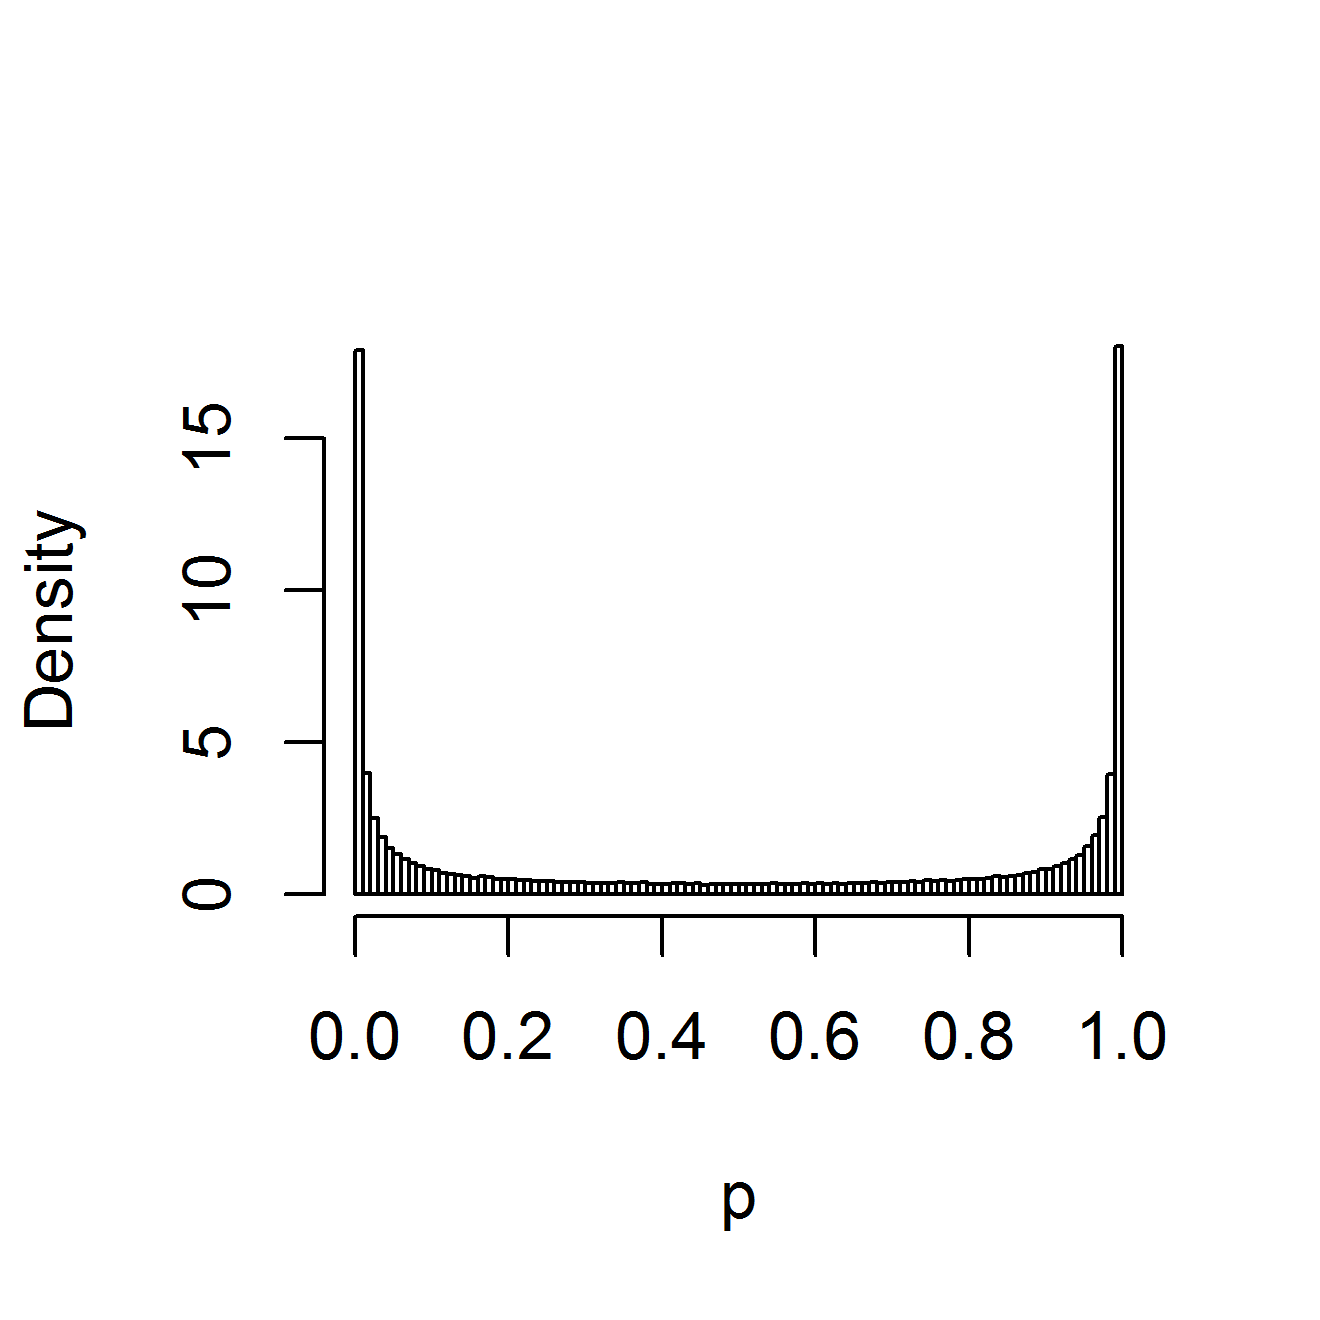
\includegraphics[height=3.3in]{Ch2-Bayes/figs/implied_prior}
\end{center}
\caption{Implied prior for $p_{0} = \exp(\beta_0)/(1+\exp(\beta_0))$ 
if $\beta_0 \sim \mbox{Normal}(0, 5^2)$.}
\label{glms.fig.impliedprior}
\end{figure}
These two priors can affect results (see sec. \ref{closed.sec.Mhbear}
for an illustration of this for a real data set), yet they are both
sensible non-informative priors. Despite this, it is often the case
that priors will have little or not impact on the results.
Choice of priors and parameterization
is very much problem-specific and often largely subjective. Moreover,
it also affects the behavior of MCMC algorithms and therefore the
analyst needs to pay some attention to this issue and possibly try
different things out.  Most standard Bayesian analysis books address
issues related to specification and affect of prior distribution
choice in some depth. Some good references include
\citet{kass_wasserman:1996}, \citet{gelman:2006} and
\citet{link_barker:2010}.


\subsection{Convergence and so-forth}
\label{glms.sec.convergence}

Once we have carried-out an analysis by MCMC, there are many other
practical issues that we have to confront. One characteristic of MCMC sampling is that Markov chains take some time to converge to their stationary distribution - in our case the posterior distribution for some parameter given  data, $[\theta|y]$. Only when the Markov chain has reached
its stationary distribution, the generated samples can be used to
characterize the posterior distribution. Thus, one of the most important issues we need to address 
is ``have the chains converged?'' Since we do not know what the
stationary posterior distribution of our Markov chain should look like
(this is the whole point of doing an MCMC approximation), we
effectively have no means to assess whether it has truly converged to
this desired distribution or not. Most MCMC algorithms only guarantee
that, eventually, the samples being generated will be from the target
posterior distribution, but no-one can tell us how long this will
take. Also, you only know the part of your posterior distribution that
the Markov chain has explored so far -- for all you know the chain
could be stuck in a local maximum, while other maxima remain
completely undiscovered.  Acknowledging that there is truly nothing we
can do to ever prove convergence of our MCMC chains, there are several
things we can do to increase the degree of confidence we have about
the convergence of our chains. Some problems are easily detected using
simple plots.  Typically a period of transience is observed in the
early part of the MCMC algorithm, and this is usually discarded as the
``burn-in'' period. The quick diagnostic to whether convergence has
been achieved is that your Markov chains look ``grassy'' -- see Fig.
\ref{glms.fig.grassy} below.  Another way to check convergence is to
update the parameters some more and see if the posterior changes. Yet
another option, and one generally implemented in {\bf WinBUGS}, is to
run several Markov chains and to start them off at different initial
values that are overdispersed relative to the posterior
distribution. Such initial values help to explore different areas of
the parameter space simultaneously; if after a while all chains
oscillate around the same average value, chances are good that they
indeed converged to the posterior distribution.
\begin{comment}
%%%%%\footnote{Running
  several parallel chains is computationally expensive. But extra
  computational demands are not the only and by no means the major
  concern some people voice when it comes to running several parallel
  MCMC chains to assess convergence. Again, consider the fact that we
  do not know anything about the true form of the posterior
  distribution we are trying to approximate. How do we, then, know how
  to pick overdispersed initial values? We don't. All we can do is
  pick overdispersed values relative to our expectations of what the
  posterior should look like. To use a quote from the home page of
  Charlie Geyer, a Bayesian statistician from the University of
  Minnesota, ``If you don't know any good starting points [...], then
  restarting the sampler at many bad starting points is [...] part of
  the problem, not part of the solution.''
  (\url{''http://users.stat.umn.edu/~charlie/mcmc/diag.html''}). His suggestion
  is that your only chance to discover a potential problem with your
  MCMC sampler is to run it for a very long time. But again, there is
  no way of knowing how long is long enough.  It is up to you to
  decide, which school of thoughts appeals more to you, one long
  versus several parallel Markov chains. Irrespectively, part of
  developing an MCMC sampler should be to make sure (within reasonable
  limits) that you are not missing regions of high posterior density
  because of the way you specify your starting values. Once you have
  explored the behavior of your chain under a reasonable range of
  starting values, you may feel comfortable enough to run only one
  long chain.}
\end{comment}
Gelman and Rubin came up with the so-called``R-hat''
statistic ($\hat{R}$) or Brooks-Gelman-Rubin statistic that
essentially compares within-chain and between-chain variance to check
for convergence of multiple chains \citep{gelman_etal:1996}. $\hat{R}$
should be close to 1 if the Markov chains have converged and
sufficient posterior samples have been obtained. In practice, $\hat{R}
= 1.2$ is probably good enough for some problems.  For some models you
can't actually realize a low $\hat{R}$. E.g., if the posterior is a
discrete mixture of distributions then you can be misled into thinking
that your Markov chains have not converged when in fact the chains are
just jumping back and forth in the posterior state-space.
%So, for example, model
%selection methods (section XYZ) sometimes suggests non-convergence.
Another situation is when one of the parameters is on the boundary of
the parameter space which might appear to be very poor mixing, but all
within some extreme region of the parameter space.\footnote{it would
  be nice if we could compile examples of this later in the book and
  reference back to this point}.
This
kind of stuff is normally ok and you need to think really hard about
the context of the model and the problem before you conclude that your
MCMC algorithm is ill-behaved.

Some models exhibit ``poor mixing'' of the Markov chains (or ``slow
convergence'') in which case the samples might well be from the
posterior (i.e., the Markov chains have converged to the proper
stationary distribution) but simply mix or move around the posterior
rather slowly. Anyway, poor mixing can happen for many reasons -- when
parameters are highly correlated (even confounded), or barely
identified from the data, or the algorithms are very terrible and
probably other reasons as well.

Slow mixing equates to high autocorrelation in the Markov chain - the
successive draws are highly correlated, and thus we need to run the
MCMC algorithm much longer to get an effective sample size that is
sufficient for estimation, or to reduce the MC error (see below) to a
tolerable level.  A strategy often used to reduce autocorrelation is
``thinning'' - i.e., keep only every $m^{th}$ value of the Markov
chain output. However, thinning is necessarily inefficient from the
stand point of inference - you can always get more precise posterior
estimates by using all of the MCMC output regardless of the level of
autocorrelation \citep{maceachern_berliner:1994,
  link_eaton:2011}. Practical considerations might necessitate
thinning, even though it is statistically inefficient. For example, in
models with many parameters or other unknowns being tabulated, the
output files might be enormous and unwieldy to work with. In such
cases, thinning is perfectly reasonable. In many cases, how well the
Markov chains mix is strongly influenced by parameterization,
standardization of covariates, and the prior distributions being
used. Some things work better than others, and the investigator should
experiment with different settings and remain calm when things don't
work out perfectly.
% MCMC is an art, as much as it is a science.


{\bf Is the posterior sample large enough?}  The subsequent samples
generated from a Markov chain are not {\it iid} samples from the
posterior distribution, due to the correlation among samples
introduced by the Markov process\footnote{In case you are not familiar
  with Markov chains, for $T$ random samples $\theta^ {(1)}$,
  ... $\theta^{(T)}$ from a Markov chain the distribution of
  $\theta^{(t)}$ depends only on the immediately preceding value,
  $\theta^{(t-1)}$.} and the sample size has to be adjusted to account
for the autocorrelation in subsequent samples (see Chapt. 8 in
\citet{robert_casella:2010} for more details). This adjusted sample
size is referred to as the effective sample size. Checking the degree
of autocorrelation in your Markov chains and estimating the effective
sample size your chain has generated should be part of evaluating your
model output. {\bf WinBUGS} will automatically return the effective
sample size for all monitored parameters. If you find that your
supposedly long Markov chain has only generated a very short effective
sample, you should consider a longer run. What exactly constitutes a
reasonable effective sample size is hard to say. A more palpable
measure of whether you've run your chain for enough iterations is the
time-series or Monte Carlo error - the ``noise'' introduced into your
samples by the stochastic MCMC process. The MC error \index{Monte
  Carlo error} is printed by default in summaries produced in the {\bf
  WinBUGS} GUI, and using the \mbox{\tt summary} command applied to
{\bf JAGS} output (MC error is called ``Time-series SE'' in {\bf
  JAGS}). You want that to be smallish relative to the magnitude of
the parameter and what smallish means will depend on the purpose of
the analysis. For a preliminary analysis you might settle for a few
percent whereas for a final analysis then certainly less than 1\% is
called for. You can run your MCMC algorithm as long as it takes to
achieve that. A consequence of the MC error is that even for the exact
same model, results will always be different. Thus, as a good rule of
thumb, you should avoid reporting MCMC results to more than 2
significant digits!
\begin{comment}
% another attempt to address this issue ineffectively 
Note that MC error in summaries of the
posterior is not the same as having an ``approximate'' solution in a
standard likelihood analysis or similar.  The approximate SE in
likelihood inference is actually wrong in its actual value.... XYZ.
\end{comment}

\subsection{Bayesian confidence intervals}

The 95\% Bayesian confidence interval based on percentiles of the
posterior is not a unique interval - there are many of them - and the
so-called ``highest posterior density'' (HPD) interval is the
narrowest interval that contains {\it at least} 95\% of the posterior
mass.  As a result (of the {\it at least} clause), for discrete
parameters, the 95\% HPD is not often exactly 95\% but usually
slightly more conservative than nominal.

\subsection{Estimating functions of parameters}

A benefit of analysis by MCMC is that we can seamlessly estimate
functions of parameters by simply tabulating the desired function of
the simulated posterior draws. For example, if $\theta$ is the
parameter of interest and let $\theta^{(i)}$ for $i=1,2,\ldots,M$ be
the posterior samples of $\theta$. Let $\eta = \exp(\theta)$, then a
posterior sample of $\eta$ can be obtained simply by computing
$\exp(\theta^{(i)})$ for $i=1,2,\ldots,M$. We give another example in
section
\ref{glms.sec.xopt}
below and throughout this book.
Almost all SCR models in this book involve at least 1 derived
parameter. For example, density $D$ is a derived parameter, being a
function of population size $N$ and the area $A$ of the underlying
state-space of the point process (see Chapt. \ref{chapt.scr0}).

\section{Bayesian Analysis using the BUGS language}

We won't be too concerned with devising our own MCMC algorithms for
every analysis
although we will do that a few times for fun.  More often, we
will rely on the freely available software package {\bf WinBUGS} or
{\bf JAGS}
for doing this.  We will always execute these {\bf BUGS} engines from
within {\bf R} using the \mbox{\tt R2WinBUGS} \citep{sturtz_etal:2005}
or, for {\bf JAGS}, the  \mbox{\tt R2jags} or 
\mbox{\tt rjags} \citep{plummer:2009} packages. 
{\bf WinBUGS} and {\bf JAGS} are  MCMC black boxes
that takes a pseudo-code description (i.e., written in the {\bf BUGS}
language) of all of the relevant stochastic
and deterministic elements of a model and generate an MCMC algorithm
for that model. But you never get to see the algorithm. Instead,
{\bf WinBUGS}/{\bf JAGS} will run the 
algorithm and  return the Markov chain output
- the posterior samples of model parameters.

The great thing about using the {\bf BUGS} language is that it forces
you to become intimate with your statistical model - you have to write
each element of the model down, admit (explicitly) all of the various
assumptions, understand what the actual probability assumptions are
and how data relate to latent variables and data and latent variables
relate to parameters, and how parameters relate to one another.

While we normally use {\bf WinBUGS}, we note that {\bf OpenBUGS} is
the current active development tree of the {\bf BUGS} project. See
\citet[][]{kery:2010} and \citet[][especially
App. 1]{kery_schaub:2011} for more on practical analysis in {\bf
  WinBUGS}.  Those books should be consulted for a more comprehensive
introduction to using {\bf WinBUGS}.  Recently we have migrated many
of our analyses to {\bf JAGS} \citep{plummer:2009}, which we adopt
later in the book. You can refer to \citet{hobbs:2011} for an
ecological introduction to {\bf JAGS}.  Next, we provide an example of
a Bayesian analysis using {\bf WinBUGS}

\subsection{Linear Regression in WinBUGS}

We provide a brief introductory example of a normal regression model
using a small simulated data set. The following commands are executed
from within your {\bf R} workspace.
First, simulate a covariate $x$ and observations $y$ having
prescribed intercept, slope and variance:
\begin{verbatim}
 x<-rnorm(10)
 mu<- -3.2+ 1.5*x
 y<-rnorm(10,mu,sd=4)
\end{verbatim}
The {\bf BUGS} model specification for a normal regression model is
written within {\bf R} as a character string input to the command
\mbox{\tt cat()} and
then dumped to a text file named \mbox{\tt normal.txt}:
\begin{verbatim}
cat("
 model {
   for (i in 1:10){
      y[i]~dnorm(mu[i],tau)        # the "likelihood"
      mu[i]<- beta0 + beta1*x[i]   # the linear predictor
     }
   beta0~dnorm(0,.01)              # prior distributions
   beta1~dnorm(0,.01)
   sigma~dunif(0,100)
   tau<-1/(sigma*sigma)            # tau is a derived parameter
}
",file="normal.txt")
\end{verbatim}
Alternatively, you
can write the model specifications directly within a text file and
save it in your current working directory, but we do not usually take
that approach in this book.

The {\bf BUGS} dialects\footnote{We use this to mean {\bf WinBUGS},
  {\bf OpenBUGS} and {\bf JAGS}} parameterize the normal distribution
in terms of the mean and inverse-variance, called the precision. Thus,
\mbox{\tt dnorm(0,.01)} implies a variance of 100.  We typically use
diffuse normal priors for mean parameters, $\beta_0$ and $\beta_1$ in
this case, but sometimes we might use uniform priors with suitable
bounds -B and +B.  Also, we typically use a $\text{Uniform}(0,B)$
prior on standard deviation parameters \citep{gelman:2006}.  But
sometimes we might use a gamma prior on the precision parameter
$\tau$.  In a {\bf BUGS} model file, every variable referenced in the
model description has to be either data, which will be input (see
below), a random variable which must have a probability distribution
associated with it using the tilde character (aka ``twiddle'')
``$\sim$'' or it has to be a derived parameter connected to variables
and data using an array: ``\mbox{\tt <-}''.


To fit the model, we need to describe various data objects to {\bf
  WinBUGS}. In particular,
we create an {\bf R} list object called \mbox{\tt data} which
are the data objects identified in the {\bf BUGS} model file.
 In the example, the
data consist of two objects which exist as $y$ and $x$ in the {\bf R}
workspace and also in the {\bf WinBUGS} model definition.
 We also have to create an {\bf R} function
that produces a list of starting values, \mbox{\tt inits}, that get sent to
{\bf WinBUGS}.
 Finally, we identify
the names of the parameters (labeled correspondingly in the {\bf WinBUGS}
model specification) that we want {\bf WinBUGS} to save the MCMC output
for. In this example, we will ``monitor'' the parameters
$\beta_0$, $\beta_1$, $\sigma$ and $\tau$.
{\bf WinBUGS} is executed using the {\bf R} command
\mbox{\tt bugs()}.
We set the option \mbox{\tt debug=TRUE} if we want the {\bf WinBUGS}
GUI to stay open (useful for analyzing MCMC output and looking at the
{\bf WinBUGS} error log). Also, we set \mbox{\tt working.dir=getwd()}
so that {\bf WinBUGS} output files and the log file are saved in the
current {\bf R} working directory.
  All of these activities together look like this:
{\small
\begin{verbatim}
 library("R2WinBUGS")    # "attach" the R2WinBUGS library
 data <- list ( "y","x")
 inits <- function()
  list ( beta1=rnorm(1),beta0=rnorm(1),sigma=runif(1,0,2) )
 parameters <- c("beta0","beta1","sigma","tau")
 out<-bugs (data, inits, parameters, "normal.txt", n.thin=2, n.chains=2,
             n.burnin=2000, n.iter=6000, debug=TRUE,working.dir=getwd())
\end{verbatim}
}

A common question is ``how should my data be formatted?'' That depends
on how you describe the model in the {\bf BUGS} language, and how your
data are input into {\bf R}.  There is no unique way to describe any
particular model and so you have some flexibility. We talk about data
format further in the context of capture-recapture models and SCR
models in Chapt. \ref{chapt.scr0} and elsewhere.  In general, starting
values are optional. We recommend to always provide reasonable
starting values where possible, both for structural parameters and
also random effects\footnote{While {\bf WinBUGS} is reasonably robust to a
  wide range of more or less plausible starting values, {\bf JAGS} is
  a lot more sensitive and especially with more complex models you
  might actually have to spend some time thinking about how to specify
  good starting values to get the model running \ref{chapt.app1}; we
  will come back to this issue when we use {\bf JAGS}}.  Note that the
previously created objects defining data, initial values and
parameters to monitor are passed to the function \mbox{\tt bugs()}.
In addition, various other things are declared: The number of parallel
Markov chains (\mbox{\tt n.chains}), the thinning rate (\mbox{\tt
  n.thin}), the number of burn-in iterations (\mbox{\tt n.burnin}) and
the total number of iterations (\mbox{\tt n.iter}).  To develop a
detailed understanding of the various parameters and settings used for
MCMC, consult a basic reference such as \citet{kery:2010}.



You should execute all of the commands given above and then look at
the resulting output (summarized in table \ref{}). Close the {\bf WinBUGS} GUI and the data will be
read back into {\bf R} (or specify \mbox{\tt debug=FALSE}).  We don't
want to give instructions on how to navigate and use the GUI - but you
can fire up {\bf WinBUGS} and read the help files, or see Ch. 4 from
\citet{kery:2010} for a brief introduction.
The print command applied to the object \mbox{\tt out} prints some
basic summary output (this is slightly edited):

{\small
\begin{verbatim}
> print(out,digits=2)
Inference for Bugs model at "normal.txt", fit using WinBUGS,
 2 chains, each with 6000 iterations (first 2000 discarded), n.thin = 2
 n.sims = 4000 iterations saved
          mean   sd  2.5%   25%   50%   75% 97.5% Rhat n.eff
beta0    -2.43 1.84 -6.21 -3.50 -2.42 -1.34  1.27    1  4000
beta1     2.62 1.54 -0.42  1.68  2.62  3.57  5.67    1  4000
sigma     5.29 1.66  3.11  4.14  4.95  6.05  9.39    1  4000
tau       0.05 0.02  0.01  0.03  0.04  0.06  0.10    1  4000
deviance 59.85 3.24 56.18 57.47 59.00 61.37 68.32    1   840

For each parameter, n.eff is a crude measure of effective sample size,
and Rhat is the potential scale reduction factor (at convergence, Rhat=1).

DIC info (using the rule, pD = Dbar-Dhat)
pD = 2.6 and DIC = 62.4
\end{verbatim}
}

 In the {\bf WinBUGS} output you see a column called ``\mbox{\tt
   Rhat}''. This is the $\hat{R}$ statistic we introduced in
 \ref{glms.sec.convergence} to check whether the multiple chains
 converged; a value near 1 indicates satisfactory convergence, which
 is indicated in the output above. DIC is the
``deviance information criterion'' \citep{spiegelhalter_etal:2002}
(see section \ref{glms.sec.modsel})
 which
some people use in a manner similar to AIC although it is recognized
to have some problems in hierarchical models \citep{millar:2009}. We
evaluate this in the context of SCR models in Chapt. \ref{chapt.gof}.

%Richard will move and write this section into Ch2
% \subsection{Modeling categorical variable effects with dummy
%   variables}
% \label{glms.sec.dummy}

% Make point here that we often have categorical variables -- with
% nominal levels these are ``factors'', and we model these using dummy
% variables but sometimes in \bugs we use ``index variables''.
%end of section Richard will develop in Ch2


\subsection{Inference about functions of model parameters}
\label{glms.sec.xopt}

Using the MCMC draws for a given model we can easily obtain the
posterior distribution of any function of model parameters.  We showed
this in the above example by providing the posterior of $\tau$ when
the model was parameterized in terms of the standard deviation $\sigma$.
 As another example, suppose that the
normal regression model above had a quadratic response function of the
form
\[
	\mathbb{E}(y_i) = \beta_0 + \beta_1 x_i + \beta_2 x_{i}^{2}
\]
Then the optimum value of $x$, i.e., that corresponding to the optimal
expected response, can be found by setting the derivative of
this function to 0 and solving for $x$. We find that
\[
df/dx = \beta_1 +
2*\beta_2 x = 0
\]
yields that $x_{opt} = -\beta_1/(2*\beta_2)$.  We can just
take our posterior draws for $\beta_1$ and $\beta_2$ and obtain a
posterior sample of $x_{opt}$ by this simple calculation applied to
the posterior output. As an exercise, take
the normal model above and simulate a quadratic response and then
describe the posterior distribution of $x_{opt}$.


\section{Model Checking and Selection}
\label{glms.sec.modsel}

In general terms model checking - or assessing the adequacy of the
model - and model selection are quite thorny issues and, despite
contrary and, sometimes, strongly held belief among practitioners, there are not
really definitive, general solutions to either problem. We're against
dogma on these issues and think people need to be open-minded about
such things and recognize that models can be useful whether or not
they pass certain statistical tests. Some models are intrinsically
better than others because they make more biological sense or foster
understanding or achieve some objective that some  bootstrap
or other goodness-of-fit test can't decide for you. That said, it
gives you some confidence if your model seems adequate in a purely statistical
sense.
We provide a very brief overview of concepts here, but provide more
detailed coverage in Chapt. \ref{chapt.gof}.
See also coverage of these topics in
\citet[][]{kery:2010} and
\citet[][]{link_barker:2010}
for specific context related to Bayesian
model checking and selection.

\subsection{Goodness-of-fit}
\label{glms.sec.gof}

Goodness-of-fit testing is an important element of any analysis
because  our model represents a general set of hypotheses
about the ecological and observation processes that generated our
data. Thus, if our model ``fits'' in some statistical or scientific
sense, then we believe it to be consistent with the hypotheses that
went into the model. More formally, we would conclude that the data
are {\it not inconsistent} with the hypotheses, or that the model
appears adequate. If we have enough
data, then of course we will reject any set of statistical hypotheses.
Conversely, we can always come up with a model that fits by making the
model extremely complex. Despite this paradox, it seems to us that
simple models that you can understand should usually be preferred even
if they don't fit, for example if they embody essential mechanisms
central to our understanding of things, or
if we think that some contributing factors to lack-of-fit are minor or
irrelevant to the scientific context and intended use of the model.
In other words, models can be useful irrespective of whether they fit
according to some formal statistical test of fit.  Yet
the tension is there to obtain fitting models, and this comes naturally at
the expense of models that can be easily interpreted and studied and
effectively used.
Unfortunately, conducting a goodness-of-fit test is
not always so easy to do. And, moreover, it is never really easy (or
especially convenient) to decide if your goodness-of-fit test is worth
anything. It might have 0 power!
Despite this,
we recommend attempting to assess model fit in real applications,
as a general rule, and we provide some basic guidance here and some more
specific to SCR models in
Chapt. \ref{chapt.gof}.

To evaluate goodness-of-fit in Bayesian analyses, we will most often
use the Bayesian p-value \citep{gelman_etal:1996}.  The basic idea is to define
a fit statistic or ``discrepancy measure'' and compare the posterior distribution of that
statistic to the posterior predictive distribution of that statistic
for hypothetical perfect data sets for which the model is known to be correct. For
example, with count frequency data, a standard measure of fit is the
sum of squares of the ``Pearson residuals'',
\[
D(y_i,\theta) = \frac{(y_i - \mathbb{E}(y_i))}{\sqrt{\mbox{Var}( y_{i} )}}
\]
The fit statistic based on the squared residuals computed from the
observations is 
\[
T({\bf y}, \theta) = \sum_{i} D(y_{i},\theta)^{2}
\]
which can be computed at each iteration of a MCMC algorithm given the
current values of parameters that determine the
 response distribution.  At the same time (i.e., at each MCMC
 iteration),
the equivalent statistic is computed for a
``new'' data set, say ${\bf y}^{new}$, 
simulated using the current parameter values. From the new data set,
we compute the same fit statistic:
\[
T({\bf y}^{new}, \theta) = \sum_{i} D(y_{i}^{new},\theta)^{2}
\]
and 
the
Bayesian p-value is simply the posterior probability $\Pr(T({\bf
  y}^{new})  >  T({\bf y}))$
 which should be close to $0.50$ for a good model -- one that
 ``fits'' in the sense that the observed data set is
 consistent with realizations simulated under the model being fitted
 to the observed data. In practice
we judge ``close to 0.50'' as being ``not too close to 0 or 1'' and,
as always, closeness is somewhat subjective. We're happy with anything
$>.1$ and $<.9$ but might settle for $>.05$ and $<0.95$. 
Another useful fit statistic is the Freeman-Tukey
statistic, in which
\[
D({\bf y},\theta) = \sum_{i} ( \sqrt{y_{i}} - \sqrt{e_{i}} )^2
\]
\citep{brooks_etal:2000}, where $y_{i}$ is the observed value of
observation $i$ and $e_{i}$ its expected value. In contrast to a
Chi-square discrepancy, the Freeman-Tukey statistic removes the need
to pool cells with small expected values.
In summary, you can see that 
the Bayesian p-value is easy to compute,
and it is widely used as a result.


\subsection{Model Selection }

In ecology, scientific hypotheses are often manifest as different models or parameters
 of a model, and so
evaluating the importance of different models is fundamental 
to many ecological studies.
For model selection we typically use three different methods: First
is, let's say, common sense. If a variable should plausibly be
relevant to explaining the data-generating processes, and it has 
 posterior mass
concentrated away from 0, then it seems like it should be regarded as
important - that is, it is ``significant.''  This approach seems to
have fallen out of favor in ecology over the last 10 or
15 years but in many situations it is a reasonable thing to do.

For regression problems we sometimes use the indicator variable method
of \citet{kuo_mallick:1998}, in 
which we introduce a set of binary variables $I_{k}$ for variable
$k$, and express the model as, e.g., for a single covariate model:
 \[
 \mathbb{E}(y_i) = \beta_0 + I_{1} \beta_1 x_{i}
\]
where $I_{1}$ is given a Bernoulli prior distribution with some prescribed
probability. E.g., $I_{1} \sim \mbox{Bernoulli}(0.50)$ to provide a prior probability
of 0.50 that variable $x$ should be an element of the linear
predictor. The posterior probability of the event $I_{1}=1$ is a gage of
the importance of the variable $x$. i.e., high values of $\Pr(I_{1}=1)$
indicate stronger evidence to support that ``$x$ is in the model''
whereas values of $\Pr(I_{1}=1)$ close to 0 suggest that $x$ is less
important.  Expansion of the model to include the binary variable
$I_{1}$ defines a set of 2 distinct models for which we can directly
compute the posterior probabilities for, merely by tallying up the
posterior frequency of $I_{1}$.

See
\citet[][Chapt. 3]{royle_dorazio:2008} for an example in the context
of logistic regression. This approach seems to even work sometimes
with fairly complex hierarchical models of a certain form. E.g.,
\citet{royle:2008} applied it to a random effects model to evaluate
the importance of the random effect component of the model.  The main
problem, which is really a general problem in Bayesian model
selection, is that its effectiveness and results will
typically be highly sensitive to the prior distribution on the
structural parameters (e.g., see \citet[][table 3.6]{royle_dorazio:2008}).
The reason for this is obvious: If $I_{1} = 0$ for the current
iteration of the MCMC algorithm, so that $\beta$ is sampled from the
prior distribution, and the prior distribution is very diffuse, then
extreme values of $\beta$ are likely. Consequently, when the current value of
$\beta$ is
far away from the mass of the posterior when $I_{1}=1$, then the Markov
chain may only jump from $I_{1}=0$ to $I_{1}=1$ infrequently.  One seemingly
reasonable solution to this problem \citep{aitkin:1991}
is to fit the full
model to obtain posterior distributions for all parameters, and then
use those as prior distributions in a ``model selection'' run of the
MCMC algorithm.  This seems preferable to more-or-less arbitrary restriction of
the prior support to improve the performance of the MCMC algorithm.

A third method that we advocate is subject-matter context. It seems
that there are some situations -- some models -- where one should not
have to do model selection because it is necessitated by the specific
context of the problem, thus rendering a formal hypothesis test
pointless \citep{johnson:1999}.  Certain aspects of SCR models are
such an example. In SCR models, we will see that ``spatial location''
of individuals is an element of the model. The simpler, reduced, model
is an ordinary capture-recapture model which is not spatially explicit
(i.e., Chapt. \ref{chapt.closed}), but it seems silly and pointless to
think about actually using the reduced model even if we could concoct
some statistical test to refute the more complex model.  The simpler
model is manifestly wrong but, more importantly, not even a plausible
data-generating model!  Other examples are when effort, area or sample
rate is used as a covariate. One might prefer to have such things in
models regardless of whether or not they pass some statistical litmus
test.
%That said, 
%although one can always find referees to argue for pedantic procedure
%over thinking.

Many problems can be approached using one of these methods but there
are also broad classes of problems that can't and, for those, you're
on your own. In later chapters (especially Chapt. \ref{chapt.gof}) we
will address model selection in specific contexts and we hope those
will prove useful for a majority of the situations you might
encounter.


\section{Poisson GLMs}
\label{glms.sec.poisson}

The Poisson GLM (also known as ``Poisson regression'') is probably the
most relevant and important class of models in all of ecology. The
basic model assumes observations $y_{i}; i=1,2,...,n$ follow a Poisson
distribution with mean $\lambda$ which we write
\[
 	y_{i} \sim \mbox{Poisson}(\lambda)
\]
Commonly $y_{i}$ is a count of animals or plants at some point in
space $i$, and $\lambda$ might depend on $i$. For example, $i$ might index point
count locations in a forest, BBS route centers, or sample quadrats, or
similar.  If covariates are available it is typical to model them as
linear effects on the log mean. If $x_i$ is some measured covariate
associated with observation $i$. Then,
\[
 	\log(x_i) = \beta_0  + \beta_1 x_i
\]

While we only specify the mean of the Poisson model directly, the
Poisson model (and all GLMs) has a ``built-in'' variance which is
directly related to the mean. In this case, $\mbox{Var}(y) = \mathbb{E}(y) =
\lambda$. Thus the model accommodates a linear increase in variance
with the mean.

%Richard: move to Ch2
% \subsection{Important properties of the Poisson distribution}
% \label{glms.sec.properties}

% There are two properties of the Poisson distribution
% that make it extremely useful in ecology. First
% is the property of {\it compound additivity}. If $y_1$ and $y_2$ are
% Poisson random variables with means $\lambda_1$ and $\lambda_2$,
% then their sum $N=y_1+y_2$ is Poisson with mean $\lambda_1+\lambda_2$. Thus,
% if the observations can be viewed as an aggregate of counts over some
% finer unit of measurement, then the Poisson mean aggregates in a corresponding
% manner. This comes in hand in some ecological applications
% where we have counts, $y_{i}$, made on sample units with different but known areas $A_{i}$. 
% Then, we might assume 
% the counts have a Poisson distribution with mean $A_{i}\lambda$. On the log-scale we see that 
% $log(A_{i})$ enters as an additive constant -- usually referred to as the ``offset'' in GLM
% lingo. 
% A second useful property of the Poisson distribution is its
% direct relationship to the multinomial.
% If $y_1$ and $y_2$ are $iid$ Poisson then,
% conditional on their sum $N = y_1 + y_2$, their joint distribution is multinomial
%  with sample size $N$ and cell probabilities
% $\lambda_1/(\lambda_1+\lambda_2)$ and
% $\lambda_2/(\lambda_1+\lambda_2)$.  As a result of this, most
% multinomial models can be analyzed as a Poisson GLM and {\it vice versa}.
%END section moved to Ch2

\subsection{Example: Breeding Bird Survey Data}

As an example we consider a classical situation in ecology where
counts of an organism are made at a collection of spatial
locations. In this particular example, we have mourning dove 
({\it Zenaida macroura})
counts
made along North American Breeding Bird Survey (BBS) routes in
Pennsylvania, USA. A route consists of 50 stops separated by 0.5
mile. For the purposes here we are defining $y_i$ = route total count
and the sample location will be marked by the center point of the BBS
route.  The survey is run annually and the data set we have is
1966-1998. BBS data can be obtained online at \mbox{\tt http:\//\//www.pwrc.usgs.gov\//bbs\//}, but the particular chunk of data we will be using here is also included in the {\tt scrbook} package ({\tt bbsdata}).
We will make use of the whole data set shortly but for now we're going
to focus on a specific year of counts -- 1990 -- for the sake of
building a simple model.
 For 1990 there were 77 active routes, where rows index the unique route, column 1 is the
route ID, columns 2-3 are the route coordinates (longitude/latitude),
column 4 is a habitat covariate ``forest cover'' (standardized, see
below) and the remaining columns are the yearly counts. Years for
which a route was not run are coded as ``\mbox{\tt NA}'' in the data matrix. We
imagine that this will be a typical format for many ecological
studies, perhaps with more columns representing covariates.  To read
in the data and display the first few elements of the data frame containing the counts, do
this:
{\small
\begin{verbatim}
data(bbsdata) #loads data frame 'bbs'
bbsdata$counts[1:2,1:6]
      X     lon    lat    habitat X66 X67
1 72002 -80.445 41.501 -0.3871372  NA  24
2 72003 -80.347 41.214 -1.0171629  NA  NA
\end{verbatim}
}

It is useful to display the spatial pattern in the observed
counts. For that we use a spatial dot plot -- where we plot the
coordinates of the observations and mark the color of the plotting
symbol based on the magnitude of the count.  We have a special
plotting function for that which is called \mbox{\tt spatial.plot()}
and it is available with the supplemental {\bf R} package \mbox{\tt
  scrbook}.  Actually, what we want to do here is plot the log-counts
(+1 of course) which (Fig. \ref{glms.fig.padovecounts}) display a
notable pattern that could be related to something. The {\bf R}
commands for obtaining this figure are: 
{\small
\begin{verbatim}
library("scrbook")
data(bbsdata)
library("maps")

y<-bbsdata$counts[,"X90"]  # pick out 1990
notna<-!is.na(y)
y<-y[notna]
locs<-bbsdata$counts[notna,c("lon","lat")]
sz<- y/max(y)

par(mar=c(3,3,3,6))
plot(locs,pch=" ",xlim=range(locs[,1])+c(-.3,+.3),ylim=c(range(locs[,2]) + c(-.6,.6)),
            axes=FALSE,xlab=" ",ylab=" ")
map('state',regions='pennsylvania',add=TRUE,lwd=2)
spatial.plot(bbsdata$counts[notna,2:3],y,cx=1+sz*6,add=TRUE)
\end{verbatim}
}
We can ponder the potential effects that
might lead to dove counts being high....corn fields, telephone wires,
barn roofs along with misidentification of pigeons, these could all
correlated reasonably well with the observed count of mourning doves.
Unfortunately we don't have any of that information.
\begin{figure}
\begin{center}
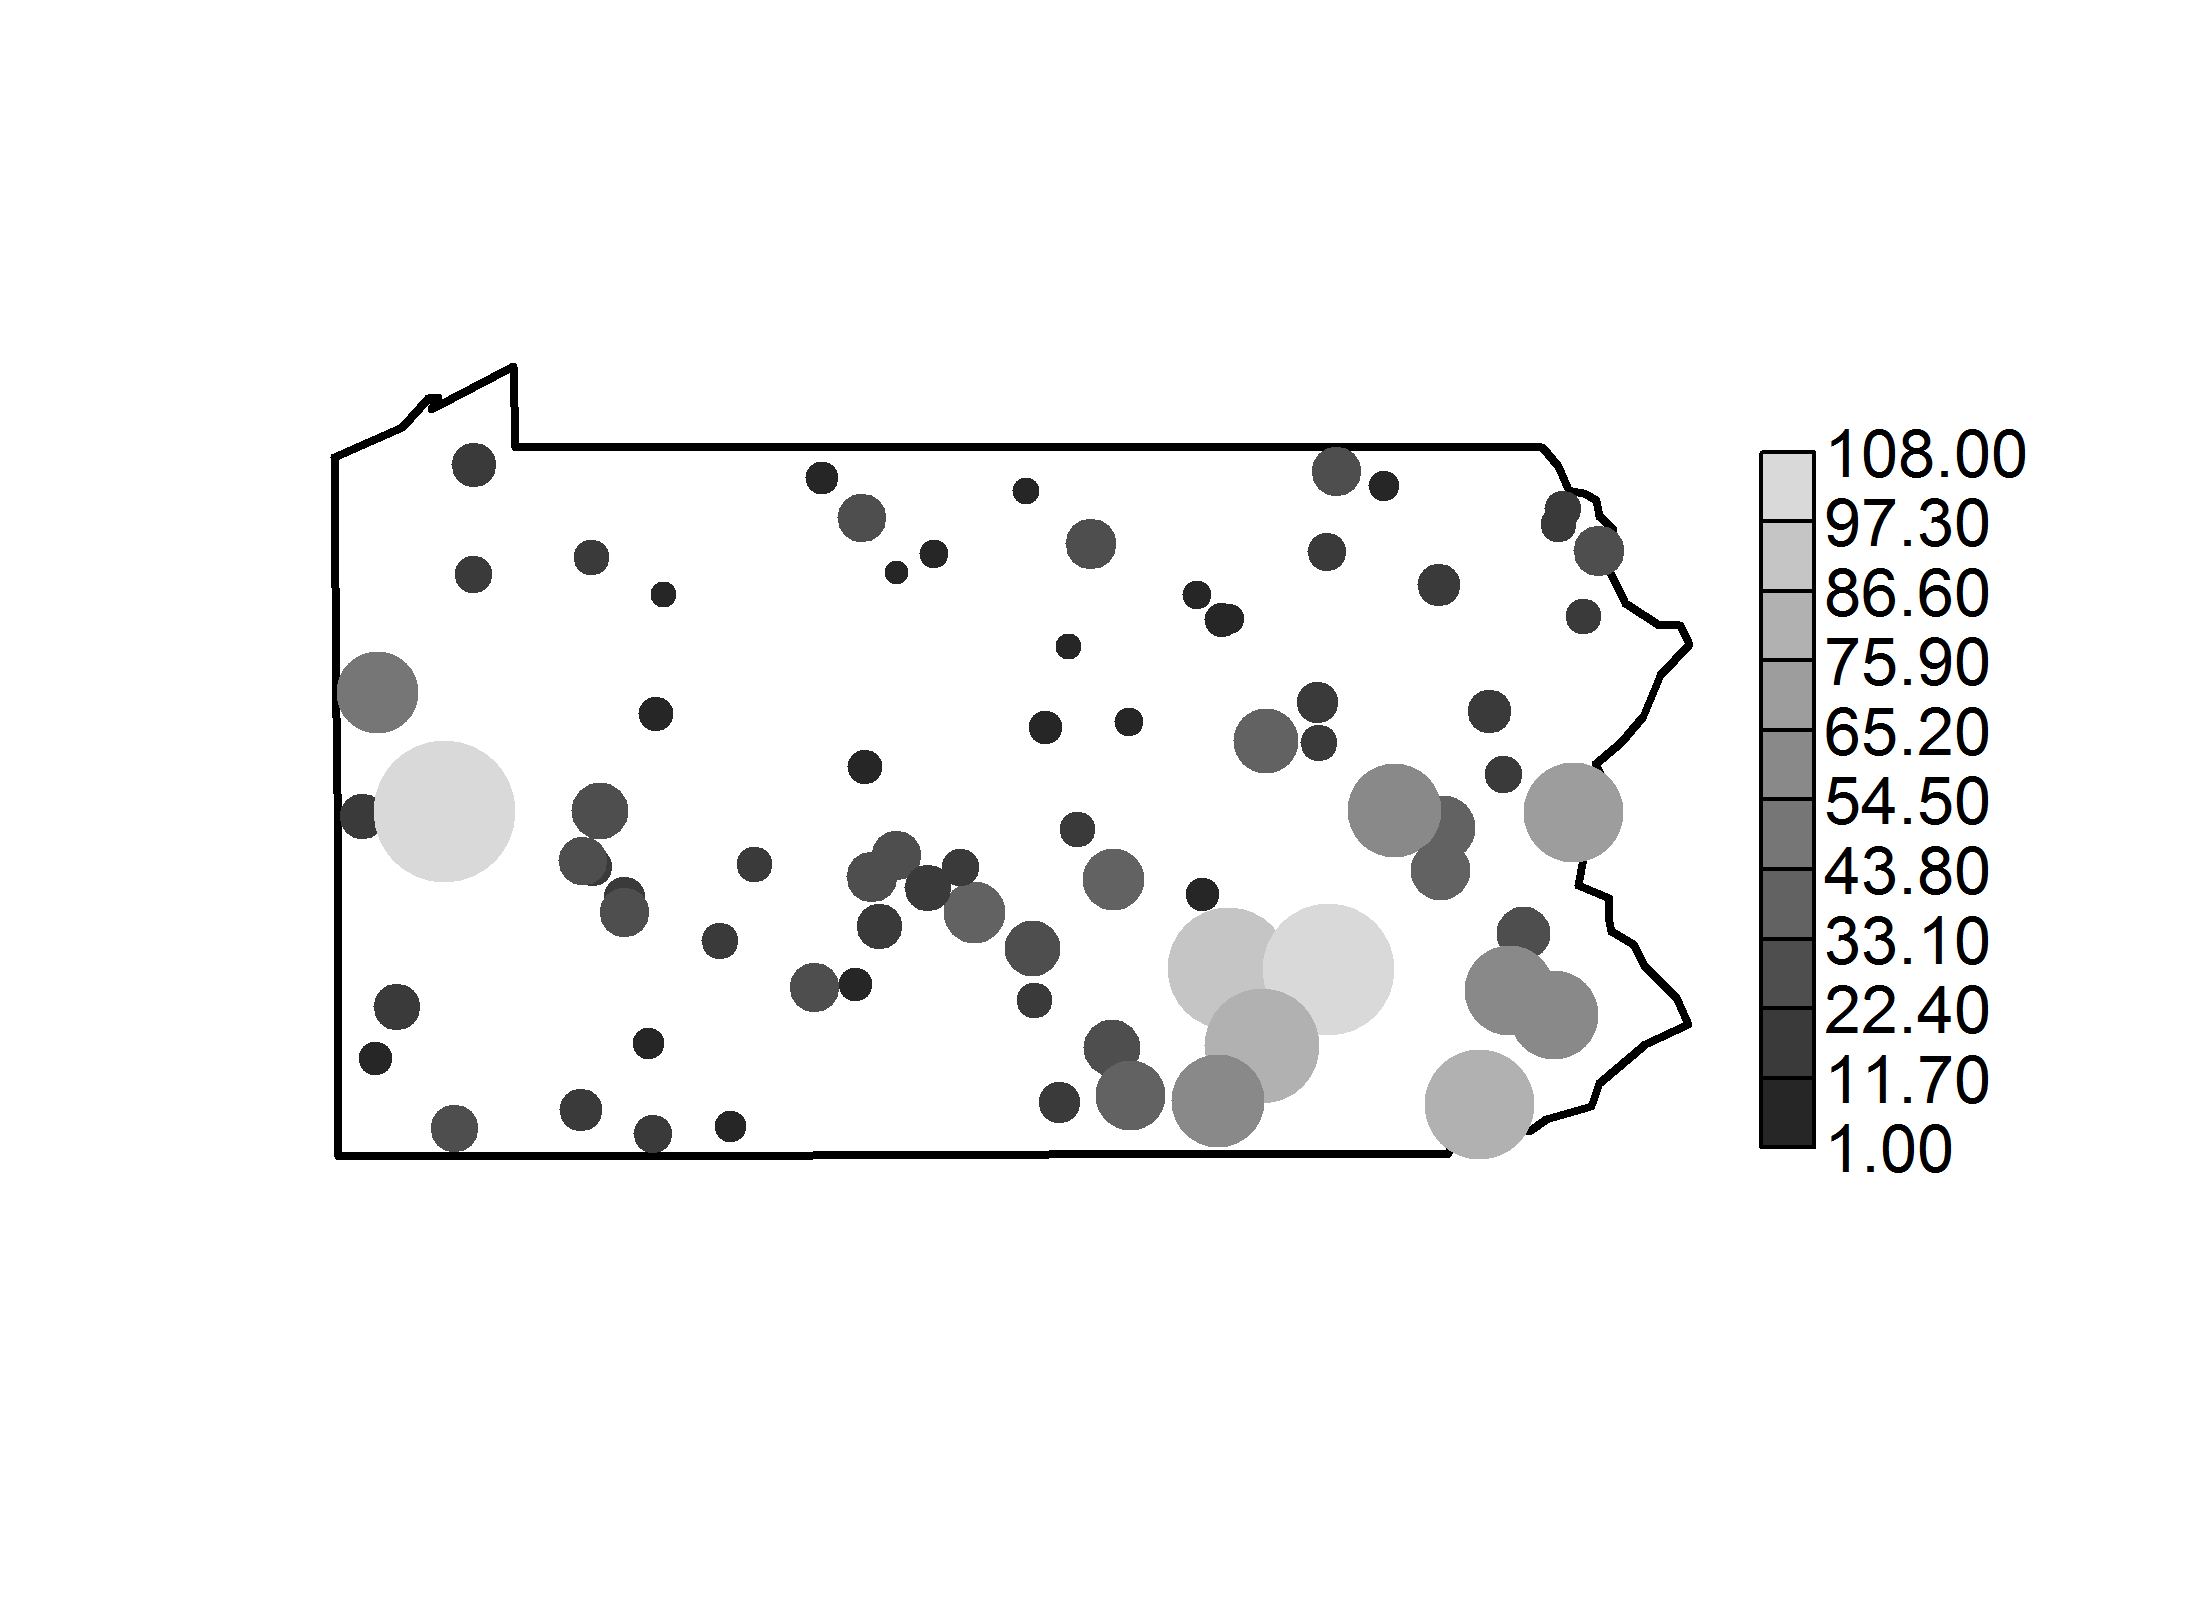
\includegraphics[height=2.75in]{Ch2-Bayes/figs/pacounts}
\end{center}
\caption{Plot  mourning doves along North American Breeding Bird
  Survey routes in Pennsylvania (year = 1990). Plot symbol shading and
  circle size is
  proportional to raw count. }
\label{glms.fig.padovecounts}
\end{figure}
However, we do have a measure of forest cover
(provided in the data frame
``\mbox{\tt bbsdata\$habitat}'') which can be plotted using the \mbox{\tt spatial.plot} function
with the following {\bf R} commands
{\small
\begin{verbatim}
habdata<-bbsdata$habitat
map('state',regions="penn",lwd=2)
I<-matrix(NA,nrow=30,ncol=40)
I<- matrix(habdata[,"dfor"],ncol=40,byrow=FALSE)
ux<-unique(habdata[,2])
uy<-sort(unique(habdata[,3]))

par(mar=c(3,3,3,6))
plot(locs,pch=" ",xlim=range(locs[,1])+c(-.3,+.3),ylim=c(range(locs[,2]) + c(-.6,.6)),axes=FALSE,xlab=" ",ylab=" ")
image(ux,uy,rot(I),add=TRUE,col=gray(seq(3,17,,10)/20) )
map('state',regions='pennsylvania',add=TRUE,lwd=3,col="white")
image.scale(I,col=gray(seq(3,17,,10)/20) )
points(locs,pch=20,col="white")
\end{verbatim}
}
where the result appears in Fig. \ref{glms.fig.paforest}.
We see a prominent pattern that indicates high forest coverage in the
central part of the state and low forest cover in the SE.  Inspecting
the previous figure of the raw counts suggests a relationship between
counts and forest cover which is perhaps not surprising.
\begin{figure}
\begin{center}
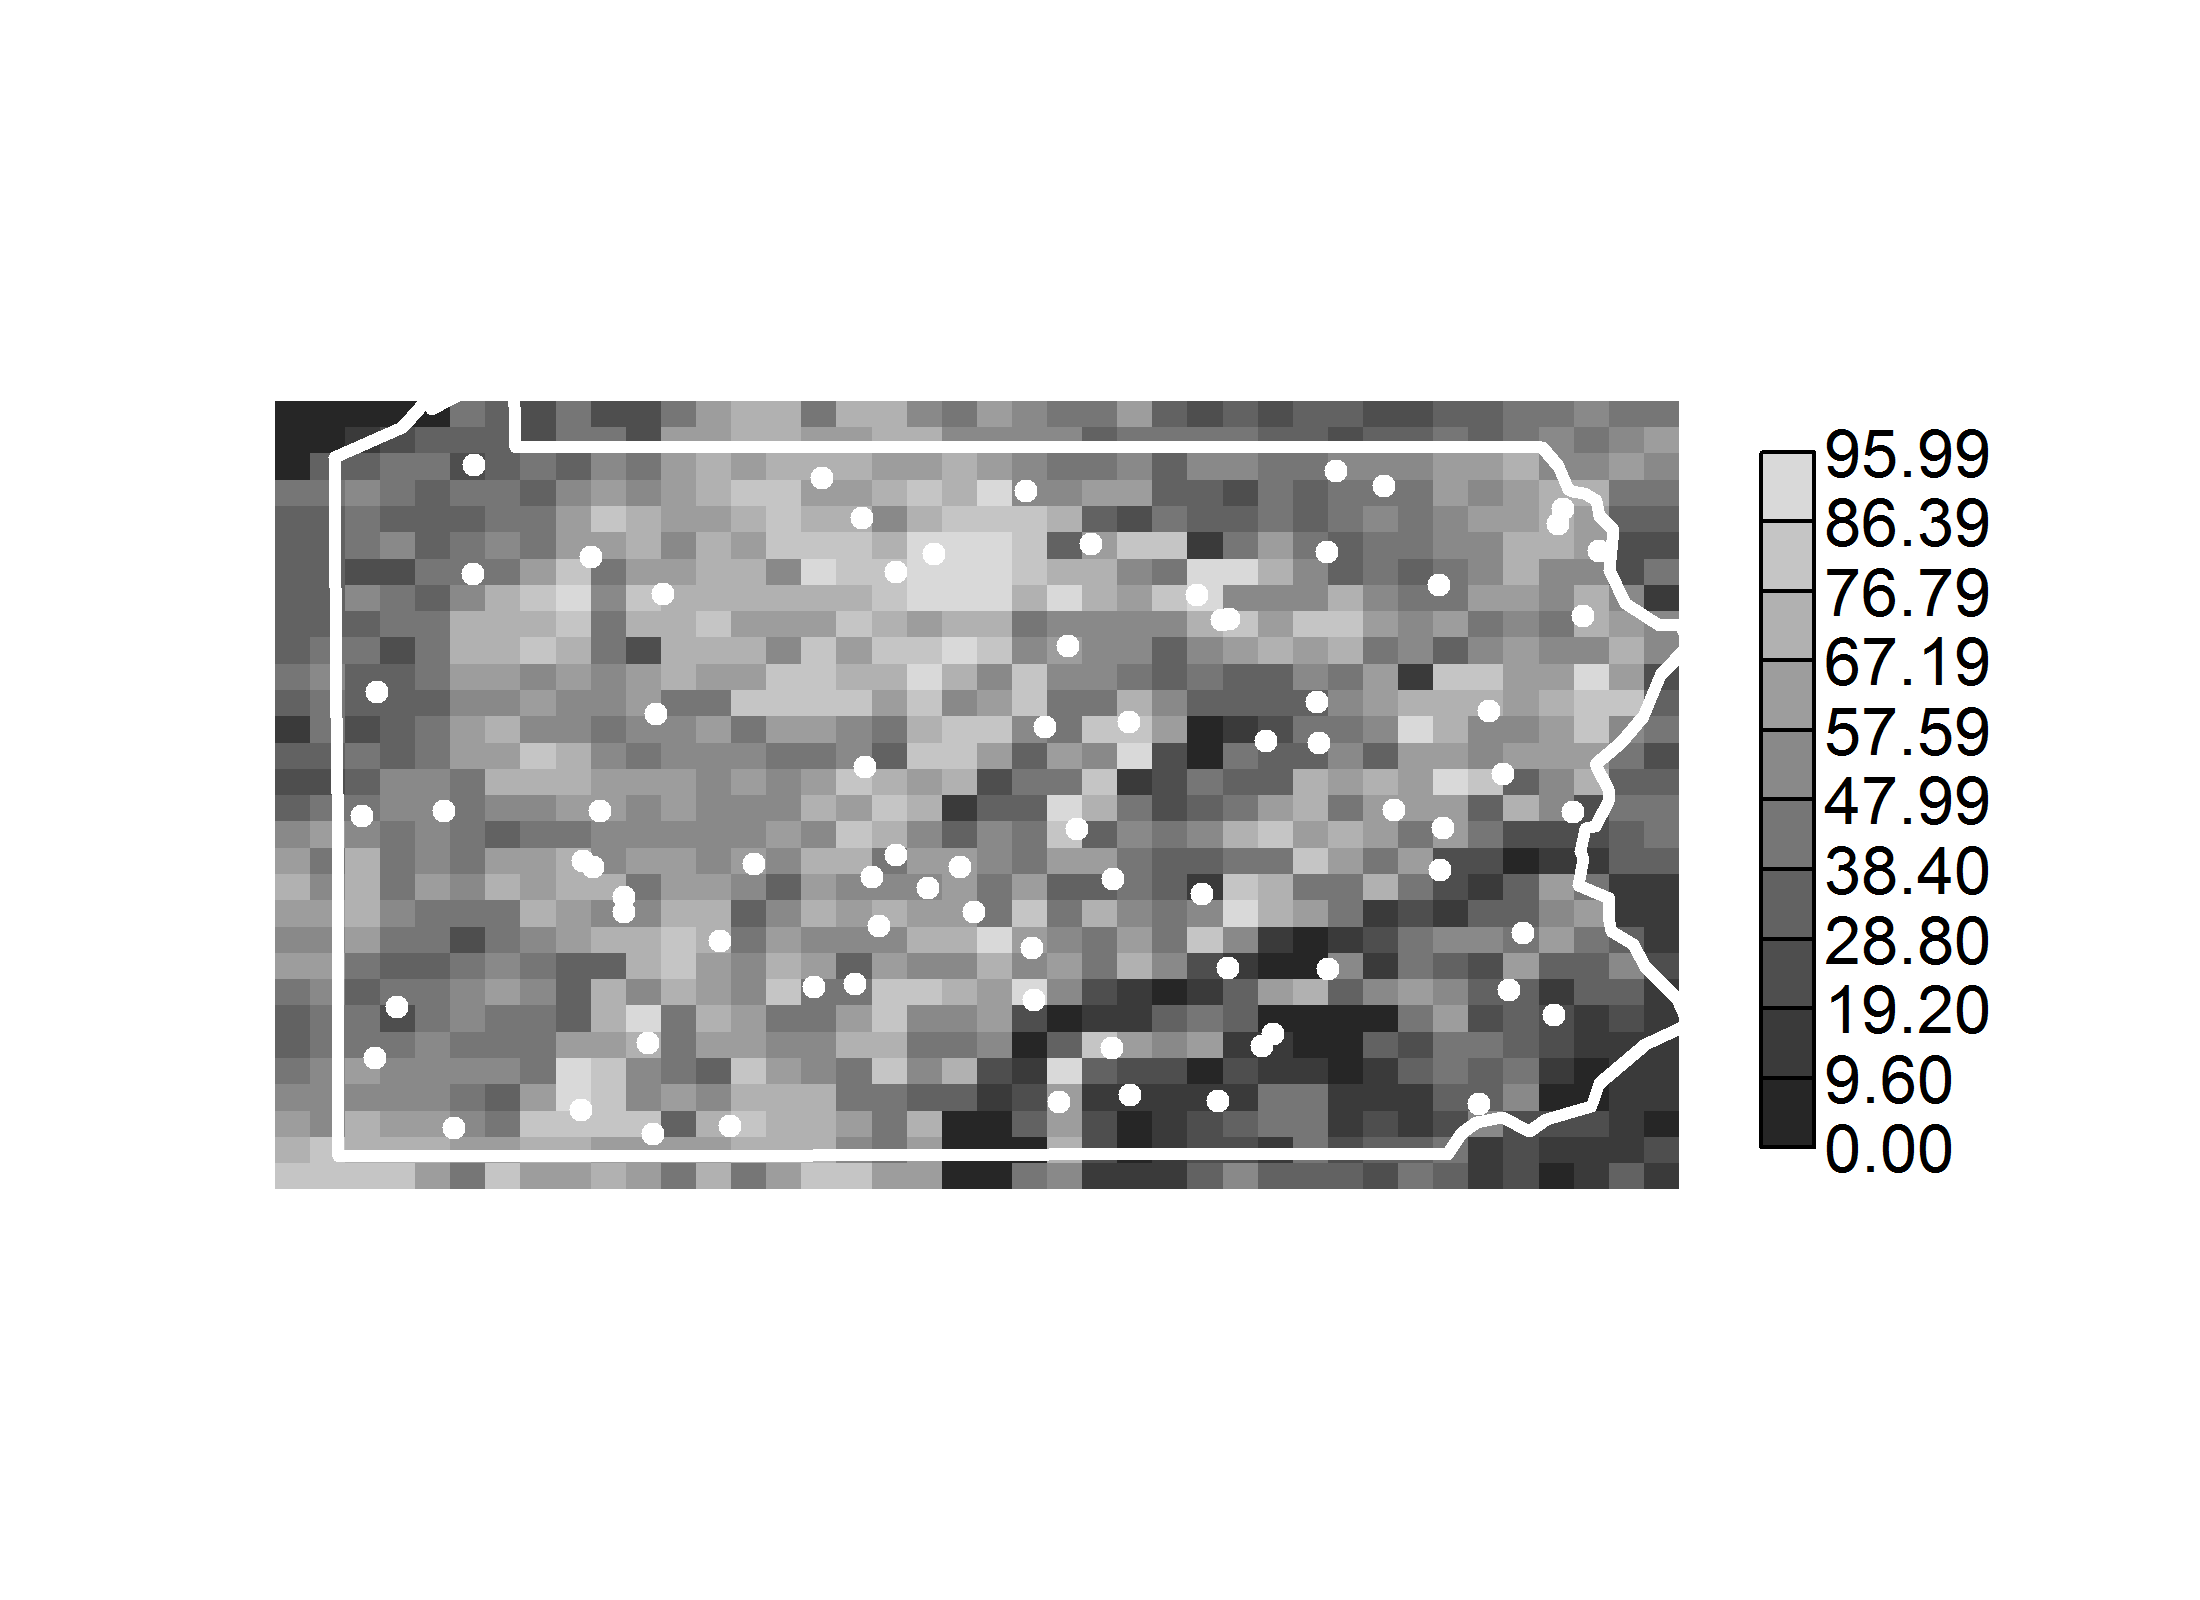
\includegraphics[height=2.75in]{Ch2-Bayes/figs/paforest}
\end{center}
\caption{Forest cover (percent deciduous) in Pennsylvania.}
\label{glms.fig.paforest}
\end{figure}

\subsection{Doing it in WinBUGS}

Here we demonstrate how to fit a Poisson GLM in {\bf WinBUGS} using the
covariate $x_{i} =$ forest cover along BBS route $i$. It is advisable that $x_i$ be
standardized in most cases as this will improve mixing of the Markov
chains. We have pre-standardized the forest cover covariate for the
BBS route locations,
 and so we don't have to worry about that
here.  To read the BBS data into {\bf R} and get things set up for
{\bf WinBUGS}
we issue the following commands:
{\small
\begin{verbatim}
library("scrbook")
data(bbsdata)

y<-bbsdata$counts[,"X90"]  # pick out 1990
notna<-!is.na(y)
y<-y[notna]
## forest cover already standardized here:
habitat<-bbsdata$counts[notna,"habitat"]
M<-length(y)

library("R2WinBUGS")                # load R2WinBUGS
data <- list ( "y","M","habitat")   # bundle data for WinBUGS
\end{verbatim}
}
Now we write out the Poisson model specification in {\bf WinBUGS}
pseudo-code, provide initial values, identify parameters to be
monitored and then execute {\bf WinBUGS}:
{\small
\begin{verbatim}
cat("
model {
    for (i in 1:M){
      y[i]~dpois(lam[i])
      log(lam[i])<- beta0+beta1*habitat[i]
     }
 beta0~dunif(-5,5)
 beta1~dunif(-5,5)
}
",file="PoissonGLM.txt")

inits <- function()  list ( beta0=rnorm(1),beta1=rnorm(1))
parameters <- c("beta0","beta1")
out<-bugs (data, inits, parameters, "PoissonGLM.txt", n.thin=2,n.chains=2,
                n.burnin=2000,n.iter=6000,debug=TRUE,working.dir=getwd())
\end{verbatim}
}
%Note the close correspondence in how the model is
%specified here compared with the normal regression model
%previously. As an exercise you should discuss the specific differences
%between the {\bf BUGS} model specifications for the normal and Poisson
%models. 

% Model output is summarized in table \ref{glms.tab.poisreg}. 
% \begin{table}
% \caption{Inference for Poisson GLM, fit using WinBUGS,
%  2 chains, each with 6000 iterations (first 2000 discarded), n.thin = 2
%  n.sims = 4000 iterations saved.}
%    \scriptsize
%   \begin{tabular}{lccccccccc}
%     \hline
%         \hline
%  Parameter &    mean   & sd   &  2.5\%    &  25\%  &    50\%   &   75\%  &  97.5\% & Rhat & n.eff \\
%      \hline
% beta0  &     3.152 & 0.025  &  3.103  &  3.135  &  3.152  &  3.168 &  3.199 & 1.001 & 4000 \\
% beta1  &    -0.497 & 0.021 & -0.537 &  -0.511 &  -0.497 &  -0.484 &  -0.456 & 1.001 & 4000 \\
% deviance & 1116.576 & 1.997 & 1115.000 & 1115.000 & 1116.000 & 1117.000 & 1122.000 & 1.002 & 4000 \\
%     \hline
%   \end{tabular}
%   \label{glms.tab.poisreg}
% \vspace{0.5cm}
% \end{table}
% since I guess this is the first BUGS analysis we might keep the actual output here. 

The {\bf WinBUGS} output can be viewed in {\bf R} using the {\tt print} command:
{\small
\begin{verbatim}
print(out,digits=3)
Inference for Bugs model at "PoissonGLM.txt", fit using WinBUGS,
 2 chains, each with 6000 iterations (first 2000 discarded), n.thin = 2
 n.sims = 4000 iterations saved
             mean    sd     2.5%      25%      50%      75%    97.5%  Rhat n.eff
beta0       3.152 0.025    3.103    3.135    3.152    3.168    3.199 1.001  4000
beta1      -0.497 0.021   -0.537   -0.511   -0.497   -0.484   -0.456 1.001  4000
deviance 1116.576 1.997 1115.000 1115.000 1116.000 1117.000 1122.000 1.002  4000
\end{verbatim}
}

% We might wonder whether this model provides an adequate fit to our
% data.  To evaluate that, we used a Bayesian p-value analysis with fit
% statistic based on the Freeman-Tukey residual by replacing the model
% specification above with this:
% {\small
% \begin{verbatim}
% cat("
% model {
%     for (i in 1:M){
%       y[i]~dpois(lam[i])
%       log(lam[i])<- beta0+beta1*habitat[i]
%       d[i]<-  pow(pow(y[i],0.5)-pow(lam[i],0.5),2)   #

%       ynew[i]~dpois(lam[i])
%       dnew[i]<-pow( pow(ynew[i],0.5)-pow(lam[i],0.5),2)

%      }
%  fit<-sum(d[])
%  fitnew<-sum(dnew[])
%  beta0~dunif(-5,5)
%  beta1~dunif(-5,5)
% }
% ",file="PoissonGLM.txt")
% \end{verbatim}
% }
% The Bayesian p-value is the proportion of times $fitnew > fit$ which,
% for this data set, is 0. This suggests that the basic Poisson model does 
% not fit well.

\subsection{ Constructing your own MCMC algorithm}
\label{GLMM.sect.mcmc}

At this point it might be helpful to suffer through an example
building a custom MCMC algorithm. Here, we develop an MCMC algorithm
for the Poisson regression model, using a Metropolis-within-Gibbs
sampling framework.  Building MCMC algorithms is covered in more
detail in Chapt. \ref{chapt.mcmc} where you can also find step-by-step
instructions for Metropolis-within-Gibbs samplers, should the
following section move through all this stuff too quickly.

We will assume that the two parameters have diffuse
normal priors, say $[\beta_0] = \mbox{Normal}(0,100)$ and
$[\beta_1]=\mbox{Normal}(0,100)$ where each has {\it standard deviation}
100 (recall that {\bf WinBUGS} parameterizes the normal in terms of $1/\sigma^{2}$).
We need to assemble the relevant elements of the model which are these
two prior distributions and the
likelihood $[{\bf y}|\beta_0,\beta_1] = \prod_{i} [y_i|\beta_0 \beta_1] $ which is,
mathematically, the product of the Poisson pmf evaluated at each $y_i$,
given particular values of $\beta_0$ and $\beta_1$.
Next, we need to identify the full conditionals
$[\beta_0|\beta_1, {\bf y}]$ and $[\beta_1|\beta_0,{\bf y}]$.  We use the all-purpose
rule for constructing full conditionals
(section \ref{glms.sec.rules})
 to discover that:
\[
 [\beta_0|\beta_1,{\bf y}] \propto \left\{ \prod_{i} [y_{i}|\beta_0,\beta_1]\right\}[\beta_0]
\]
Mathematically, the full conditional is of the form
\[
 [\beta_0|\beta_1,{\bf y}] \propto
\prod_{i} \left\{
\exp(-\exp(\beta_{0} + \beta_{1} x_{i}))
\exp(\beta_{0} + \beta_{1} x_{i})^{y_{i}}
\right\}
\exp(-\frac{\beta_{0}^2}{2*100})
\]
which you can program as an {\bf R} function with arguments
$\beta_{0}$, $\beta_{1}$ and ${\bf y}$ without difficulty.
The full-conditional for $\beta_{1}$ is:
\[
 [\beta_1|\beta_0,{\bf y}] \propto \left\{ \prod_{i}
   [y_{i}|\beta_0,\beta_1]\right\} [\beta_1]
\]
which has a similar mathematical representation except the prior is
expressed in terms of $\beta_{1}$ instead of $\beta_{0}$.
Remember, we could replace the ``$\propto$'' with ``$=$'' if we
put $[y|\beta_1]$ or $[y|\beta_0]$ in the denominator. But, in general,
$[y|\beta_0]$ or $[y|\beta_1]$ will be quite a pain to compute and, more
importantly, it is a constant as far as the operative parameters
($\beta_0$ or $\beta_1$,
respectively) are concerned. Therefore,
the MH acceptance probability will be the ratio of the
full-conditional evaluated at a candidate draw to that evaluated at the
current value, and so the denominator required to change $\propto$ to $=$
winds up canceling from the MH acceptance probability.
Here we will
use the so-called random walk candidate generator, which is a Normal proposal distribution, so that, for example,
 $\beta_0^{*} \sim \mbox{Normal}(\beta_0^{t},\delta)$ where $\delta$ is
 the standard-deviation of the proposal distribution, which is just a
 tuning parameter that is set by the user and adjusted to achieve
 efficient mixing of chains (see sec. \ref{mcmc.sec.mh}).
We remark also that calculations are often done on the log-scale to
preserve numerical integrity of things when quantities evaluate to
small or large numbers, so keep in mind, for example,
$a*b = \exp(\log(a) + \log(b))$ for two positive numbers $a$ and $b$.
 The ``Metropolis within
Gibbs'' algorithm for a Poisson regression turns out to be remarkably
simple and is given in Panel \ref{glms.panel.poisreg}. It is also part
of the {\tt scrbook} package and you can run 1000 iterations of it by
calling {\tt PoisGLMBBS(y=y, habitat=habitat, niter=1000)} (note that
{\tt y} = point count data and {\tt habitat} = forest cover have to
be defined in your {\bf R} workspace as shown in  the previous
analysis of these data).

\begin{panel}[htp]
\centering
\rule[0.15in]{\textwidth}{.03in}
%\begin{minipage}{2.5in}
{\small
\begin{verbatim}
set.seed(2013)  # so we all get the same result

out<-matrix(NA,nrow=1000,ncol=2)   # matrix to store the output
beta0<- -1                         # starting values
beta1 <- -.8

# begin the MCMC loop ; do 1000 iterations
for(i in 1:1000){

# update the beta0 parameter
lambda<- exp(beta0+beta1*habitat)
lik.curr<- sum(log(dpois(y,lambda)))
prior.curr<- log(dnorm(beta0,0,100))
beta0.cand<-rnorm(1,beta0,.05)         # generate candidate
lambda.cand<- exp(beta0.cand + beta1*habitat)
lik.cand<- sum(log(dpois(y,lambda.cand)))
prior.cand<- log(dnorm(beta0.cand,0,100))
mhratio<- exp(lik.cand +prior.cand - lik.curr-prior.curr)
if(runif(1)< mhratio)
     beta0<-beta0.cand

# update the beta1 parameter
lik.curr<- sum(log(dpois(y,exp(beta0+beta1*habitat))))
prior.curr<- log(dnorm(beta1,0,100))
beta1.cand<-rnorm(1,beta1,.25)
lambda.cand<- exp(beta0+beta1.cand*habitat)
lik.cand<- sum(log(dpois(y,lambda.cand)))
prior.cand<- log(dnorm(beta1.cand,0,100))
mhratio<- exp(lik.cand + prior.cand - lik.curr - prior.curr)
if(runif(1)< mhratio)
     beta1<-beta1.cand

out[i,]<-c(beta0,beta1)             # save the current values
}


plot(out[,1],ylim=c(-1.5,3.3),type="l",lwd=2,ylab="parameter value",
     xlab="MCMC iteration")
lines(out[,2],lwd=2,col="red")
\end{verbatim}
}
%\end{minipage}
\rule[-0.15in]{\textwidth}{.03in}
\caption{
{\bf R} code to run a Metropolis sampler on a simple Poisson regression model.
}
\label{glms.panel.poisreg}
\end{panel}

The first 300 iterations of the MCMC history of each parameter
are shown in Fig. \ref{glms.fig.poissonmcmc2}. These chains are
not very appealing but a couple of things are evident: 
We see
that the burn-in takes about 250 iterations and that after that chains seem to mix 
reasonably well, although this is not so clear given the scale of the
y-axis, which we have chosen to get both variables on the same graph.
We generated 10,000 posterior samples,
discarding the first 500 as burn-in, and the result is shown in
Fig. \ref{glms.fig.grassy}, this time separate panels for each
parameter.
The ``grassy''
look of the MCMC history is diagnostic of Markov chains that are
well-mixing and we would generally be very satisfied with results that
look like this.

\begin{figure}
\begin{center}
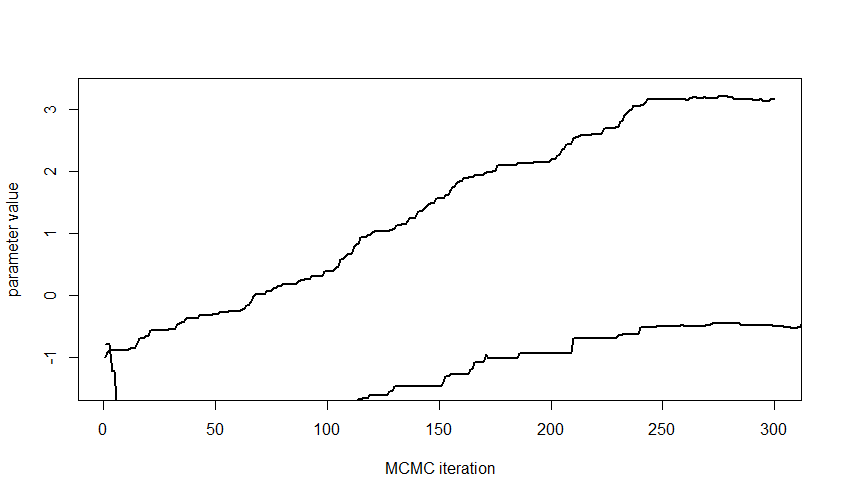
\includegraphics[height=3in,width=4in]{Ch2-Bayes/figs/poissonmcmc2}
\end{center}
\caption{First 300 MCMC iterations for the Poisson GLM model
  parameters $\beta_0$ (top)
and $\beta_1$ (bottom) using
a Metropolis-Hastings tuning parameter of
 $\delta = 0.05$.}
\label{glms.fig.poissonmcmc2}
\end{figure}

\begin{figure}
\begin{center}
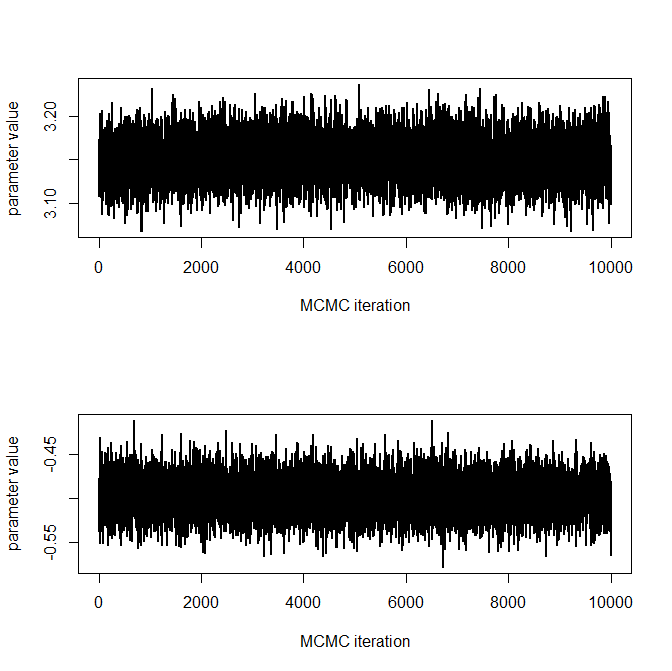
\includegraphics[height=4in,width=5in]{Ch2-Bayes/figs/poissonmcmc3}
\end{center}
\caption{Nice grassy plots of 10,000 MCMC iterations for the Poisson
  GLM model parameters $\beta_0$ (top) and $\beta_1$ (bottom) using a
  Metropolis-Hastings tuning parameter of $\delta = 0.05$.}
\label{glms.fig.grassy}
\end{figure}

Note that we used a specific set of starting values for these
simulations. It should be clear that starting values closer to the
mass of the posterior distribution might cause burn-in to occur
faster. 
%Further, for the diffuse normal prior distributions
%here we could leave the prior contribution out of the full conditional
%evaluation since it is locally constant, i.e., constant in the vicinity of
%the posterior mass, and thus has no practical effect. Removing the
%prior contribution from the MH acceptance probability is equivalent to
%saying that the parameters have an improper uniform prior, i.e.,
%$\beta_0 \sim \mbox{const}$, which is commonly used for mean parameters
%in practice.
Note also that we have
used a different prior than in our {\bf WinBUGS} model specification
given previously. We encourage you to evaluate 
 whether this seems to affect the result.

\section{Poisson GLM with Random Effects}

In most of this book, we will be dealing with random
effects in GLM-like models - similar to what
are usually referred to as generalized
linear mixed models (GLMMs). We provide a brief introduction of such a
model by way of
example, extending our Poisson regression model to include a random effect.


{\bf The Log-Normal mixture:} The classical situation involves a GLM
with a normally distributed random effect that is additive on the
linear predictor. For the Poisson case, we have:
\[
 	\log(\lambda_{i}) = \beta_0  + \beta_1 x_{i} + \eta_{i}
\]
where $\eta_{i} \sim \mbox{Normal}(0,\sigma^{2})$.  
%A natural
%alternative is to have multiplicative gamma-distributed noise,
%$exp(\eta_{i}) \sim \mbox{Gamma}(a,b)$ which would correspond to a
%negative binomial kind of over-dispersion, implying a different
%mean/variance relationship to the log-normal mixture (the interested
%reader should work that out).  Choosing between such possibilities is
%not a topic we will get into here because it doesn't seem possible to
%provide general guidance on it.   
%% For this model we carried-out a
%% goodness-of-fit evaluation using the Bayesian p-value based on a
%% Pearson residual statistic. See also \citep[][ch. 18]{kery:2010} for
%% an example involving a binomial mixed model\footnote{Kery has noticed
%%   that such tests probably have 0 power. Should use the marginal
%%   frequency of the data}. 
It is really amazingly simple to
express this model in the {\bf BUGS} language and have {\bf WinBUGS}
(or {\bf JAGS}, etc..) draw
samples from the posterior distribution. The code for analysis of the
BBS dove counts is given as follows:
the BBS dove counts: 
{\small
\begin{verbatim}
library("scrbook")
data(bbsdata)
### grab the BBS Data as before
###
### set random seed so that results are repeatable
set.seed(2013)

cat("
model {
  for (i in 1:M){
     y[i]~dpois(lam[i])
     log(lam[i])<- beta0+ beta1*habitat[i] + eta[i]
     frog[i]<-beta1*habitat[i] + eta[i]
     eta[i] ~ dnorm(0,tau)
   }

 beta0~dunif(-5,5)
 beta1~dunif(-5,5)
 sigma~dunif(0,10)
 tau<-1/(sigma*sigma)
}

",file="model.txt")

data <- list ("y","M","habitat")
inits <- function()
  list ( beta0=rnorm(1),beta1=rnorm(1),sigma=runif(1,0,4))
parameters <- c("beta0","beta1","sigma","tau")
library("R2WinBUGS")                # load R2WinBUGS library

out<-bugs (data, inits, parameters, "model.txt", n.thin=2,n.chains=2,
 n.burnin=1000,n.iter=5000,debug=TRUE)
\end{verbatim}
}

This produces the posterior summary statistics given in table \ref{glms.tab.bbspoisreg}. 
One thing we notice is
that the posterior standard deviations of the regression parameters
are much higher, a result of the extra-Poisson variation allowed for
by this model. We would also
notice much less precise predictions of hypothetical new
observations.



\begin{table}
\caption{Inference for Poisson GLM with habitat effect for mourning
  dove counts across BBS routes in PA, 1990, fit using 
{\bf WinBUGS},
 2 chains, each with 5000 iterations (first 1000 discarded), n.thin = 2
 n.sims = 4000 iterations saved.}
   \scriptsize
  \begin{tabular}{lccccccccc}
    \hline
        \hline
 Parameter &    mean   & sd   &  2.5\%    &  25\%  &    50\%   &   75\%  &  97.5\% & Rhat & n.eff \\
     \hline
$\beta_0$   &   2.98 & 0.08 &  2.82 &  2.93  & 2.98 &  3.03 &  3.12 & 1.00 & 1400 \\
$\beta_1$   &  -0.53 & 0.07 & -0.68 & -0.58 & -0.53 & -0.49 & -0.38 & 1.01 &  350 \\
$\sigma$   &   0.60 & 0.06 &  0.49 &  0.56 &  0.59 &  0.64 &  0.73 & 1.00 & 2000 \\
$\tau$     &   2.88 & 0.57 &  1.88 &  2.47 &  2.86 &  3.24 &  4.12 & 1.00 & 2000 \\
deviance & 445.94 & 12.18 & 424.00 & 437.40 & 445.20 & 453.90 & 471.50 & 1.00 & 4000 \\
    \hline
  \end{tabular}
  \label{glms.tab.bbspoisreg}
\vspace{0.5cm}
\end{table}


% {\small
% \begin{verbatim}
% print(out,digits=2)
% Inference for Bugs model at "model.txt", fit using WinBUGS,
%  2 chains, each with 5000 iterations (first 1000 discarded), n.thin = 2
%  n.sims = 4000 iterations saved
%            mean    sd   2.5%    25%    50%    75%  97.5% Rhat n.eff
% beta0      2.98  0.08   2.82   2.93   2.98   3.03   3.12 1.00  1400
% beta1     -0.53  0.07  -0.68  -0.58  -0.53  -0.49  -0.38 1.01   350
% sigma      0.60  0.06   0.49   0.56   0.59   0.64   0.73 1.00  2000
% tau        2.88  0.57   1.88   2.47   2.86   3.24   4.12 1.00  2000
% deviance 445.94 12.18 424.00 437.40 445.20 453.90 471.50 1.00  4000

% [... some output deleted ...]
% \end{verbatim}
%}
% The Bayesian p-value for this model is
% \begin{verbatim}
% > mean(out$sims.list$fit>out$sims.list$fitnew)
% [1] 0.4815
% \end{verbatim}
% indicating a pretty good fit. Given the site-level random effect, it
% would be surprising for this model to not fit! 




\section{Binomial GLMs}

Another extremely important class of models in ecology are
binomial models. We use binomial models for count data whenever the
observations are counts or frequencies and it is natural to condition
on a ``sample size'', say $K$, the maximum frequency possible in a sample.
 The random variable, $y \le K$, is then the
frequency of occurrences out of $K$ ``trials''. The parameter of the binomial
models is $p$, often called ``success probability'' which is related
to the expected value of $y$ by $\mathbb{E}(y) = pK$. Usually we are interested
in modeling covariates that affect the parameter $p$, and such models
are called binomial GLMs , binomial
regression models or logistic regression, although logistic regression
 really only applies when the logistic link is used to model
the relationship between $p$ and covariates (see below).

One of the most typical binomial GLMs occurs when the sample size
equals 1 and the outcome, $y$, is ``presence'' ($y=1$) or ``absence''
($y=0$) of a species. This is a classical species distribution
modeling situation. A special situation occurs when presence/absence
is observed with error \citep{mackenzie_etal:2002,tyre_etal:2003}.
In that case, $K>1$ samples
are usually needed for effective estimation of model parameters.

 In standard binomial regression problems the sample size
is fixed by design but interesting models also arise when the sample
size is itself a random variable. These are the $N$-mixture models
\citep{royle:2004biom, kery_etal:2005, royle_dorazio:2008, kery:2010}
and related models (in this case, $N$ being the sample size,
which we labeled $K$ above)\footnote{Some of the jargon is actually a little
bit confusing here
because the binomial index is customarily referred to as ``sample size''
but in the context of $N$-mixture models $N$ is actually the
``population size''}.
Another
situation in which the binomial sample size is ``fixed'' is closed
population capture-recapture models in which a population of
individuals is sampled $K$ times.  The number of times each individual
is encountered is a binomial outcome with parameter (encounter
probability) $p$, based on a sample of size $K$.  In addition, the
total number of unique individuals observed, $n$, is also a binomial
random variable based on population size $N$.  We consider such
models in Chapt. \ref{chapt.closed}.


\subsection{Binomial regression}

In binomial models, covariates are modeled on a suitable
transformation (the link function) of the binomial success
probability, $p$.  Let $x_{i}$ denote some measured covariate for
sample unit $i$ and let $p_{i}$ be the success probability for unit or
subject $i$.
The standard choice is the logit link function (\ref{glms.sec.glmms})
but there are many other possible link functions. 
%However, ecologists seem
%to adopt the logit link function without question in most
%applications\footnote{a notable exception is distance sampling, which
%  is all about choosing among link functions}.  
We sometimes use the
complementary log-log (= ``cloglog'') link function in ecological
applications because it is natural in some cases when the response
should scale in relation to area or effort
\citep[][p. 150]{royle_dorazio:2008}. As an example, the
``probability of observing a count greater than 0'' under a Poisson
model is $\Pr(y>0) = 1-\exp(- \lambda)$. In that case, for the
$i^{th}$ observation,
\[
\mbox{cloglog}(p_{i}) = \log(- \log(1-p_{i})) = \log(\lambda_{i})
\]
So that if you have covariates in your linear predictor for $\mathbb{E}(y)$
under a Poisson model then they are linear on the complementary
log-log link of $p$.
In models of species occurrence it seems natural to view occupancy as
being derived from local abundance $N$
\citep{royle_nichols:2003,royle_dorazio:2006,dorazio:2007}.
Therefore,
models of local abundance in which $N_{i} \sim \mbox{Poisson}(A_{i} \lambda_{i})$
for a habitat patch of area $A_{i}$ implies a model for occupancy $\psi_{i}$
of the form
\[
 \mbox{cloglog}(\psi_{i}) = log(A_{i}) + \log(\lambda_{i}).
\]
We will use the cloglog link in some analyses of
SCR models in Chapt. \ref{chapt.scr0} and elsewhere.


\subsection{ Example: Waterfowl Banding Data}

The standard binomial modeling problem in ecology is that of 
modeling species distributions, 
 where $K=1$ and the outcome is occurrence ($y=1$) or not
($y=0$) of some species. Such examples abound in books (e.g.,
\citet[][ch. 3]{royle_dorazio:2008}; \citet[][ch. 21]{kery:2010};
\citet[][ch. 13]{kery_schaub:2011}) and in the literature.
Therefore, instead, we will
consider an example involving band returns of waterfowl in the upper great plains including some Canadian provinces, which were
analyzed by \citet{royle_dubovsky:2001}.

For these data, $y_{it}$ is the number of mallard ({\it Anas platyrhynchos}) bands recovered out
of $B_{it}$ birds banded at some location ${\bf s}_{i}$ in year $t$. In this case $B_{it}$ is
fixed. Thinking about recovery rate as being proportional to harvest
rate, we use these data to explore geographic gradients in recovery rate
resulting from variability in harvest pressure experienced by
populations depending on their migration ecology. As such, we fit a
basic binomial GLM with a linear response to geographic coordinates
(including an interaction term). 
% The data ({\tt mallarddata}) are provided with the {\bf
%   R} package \mbox{\tt scrbook}. XXX MAYBE ADD LATER XXXX
Here we
 provide the part of the script for creating the model and fitting the
 model in
{\bf WinBUGS}.
There are few structural differences between this model and the
Poisson GLM fitted previously. The main things are due to the data
structure (we have a matrix here instead of a vector) and otherwise we
change the  distributional assumption to binomial (specified with
\mbox{\tt dbin}) and then use the \mbox{\tt logit} function to relate
the parameter $p_{it}$ to the covariates.  

{\flushleft \bf Dummy variables in BUGS: } In
Chapt. \ref{chapt.modeling} we introduced the concept of categorical
variables and how to display them in model formulas in the form of
``dummy variables''. In the mallard example, we model the band
recovery probability $p_{it}$ not only as a linear function (on the logit
scale) of geographic location, but also allow for variation in $p_{it}$
with year, $t$; $t=1,2,...T$. In this particular example there are
$T=5$ years of data and if we wanted to describe the full mallard
model with a formula adopting the dummy variable format, it would look
like this:

\begin{eqnarray*}
y_{it} &\sim & \mbox{Binomial}(p_{it}, B_{it}) \\
\mbox{logit}(p_{it}) &=& \beta_0 + \beta_1 x_{2t}+ \beta_2 x_{3t} +
\beta_3 x_{4t} + \beta_4 x_{5t} + 
\beta_5 \mbox{\tt lat}_i + \beta_6 \mbox{\tt lon}_i + \beta_7
\mbox{\tt lat}_i \mbox{\tt lon}_i
\end{eqnarray*}
Here, $x_{2}$ to $x_{5}$ are the dummy variable vectors of length $T$ that take on the value of 1 when $t$ corresponds to the respective year and 0 otherwise. $\beta_0$ is the common intercept term and correspond to $t=1$; $\beta_1$ - $\beta_4$ describe the difference in $p_{it}$ for each $t$ \emph{relative to} $t=1$.

There is a more concise way of implementing such a model with a
categorical covariate in {\bf BUGS}, namely, by using indexing instead
of dummy variables\footnote{Actually, in some cases a model may mix or
  converge better depending on whether you choose a dummy variable or
  an indexing description of it, although they are structurally
  equivalent \citep{kery:2010}}. Essentially, instead of estimating
the difference in $p$ relative to category 1, we estimate a separate
intercept term for each category, so that we have 5 different $\beta_0$
parameters indexed by $t$. This reduces the linear predictor to:
\[
logit(p_{it}) = \beta_{0t} +  \beta_5 \mbox{\tt lat}_i + \beta_6
\mbox{\tt lon}_i + \beta_7 \mbox{\tt lat}_i \mbox{\tt lon}_i
\]
The model can be implemented in the {\bf BUGS} language for the
mallard banding data using the following {\bf R} script, provided in
the \mbox{\tt scrbook} package (see \mbox{\tt help(mallard)}): 
{\small
\begin{verbatim}
library("scrbook")
data(mallard)    # load mallard data

sink("model.txt")
cat("
model {
 for(t in 1:5){
    for (i in 1:nobs){
       y[i,t] ~ dbin(p[i,t], B[i,t])
       logit(p[i,t]) <- beta0[t] + beta1*X[i,1] + beta2*X[i,2] + beta3*X[i,1]*X[i,2]
     }
 }
	beta1~dnorm(0,.001)
	beta2~dnorm(0,.001)
	beta3~dnorm(0,.001)
	for(t in 1:5){
 	beta0[t] ~ dnorm(0,.001)  
        }
}
",fill=TRUE)
sink()

library("R2WinBUGS")
data <- list(B=mallard$bandings, y=mallard$recoveries,
             X=mallard$locs,nobs=nrow(mallard$locs))
inits <- function(){ list(beta0=rnorm(5),beta1=0,beta2=0,beta3=0) }
parms <- list('beta0','beta1','beta2','beta3')
out <- bugs(data,inits, parms,"model.txt",n.chains=3,
 	n.iter=2000,n.burnin=1000,n.thin=2, debug=TRUE)
\end{verbatim}
}

\begin{table}
\caption{Posterior summaries for the binomial GLM of mallard band
  recovery rate.  Model contains year-specific intercepts
  ($\beta_{0t}$) and a linear response surface with interaction. 
Model was fit using {\bf WinBUGS}, and posterior summaries are based 
on 3 chains, each with 2000 iterations (first 1000 discarded), n.thin = 2
 n.sims = 1500 iterations saved.
   }
   \scriptsize
  \begin{tabular}{lccccccccc}
    \hline
        \hline
 Parameter &    mean   & sd   &  2.5\%   &    50\%   &   97.5\% & Rhat & n.eff \\
     \hline
beta0[1] &  -2.346& 0.036&   -2.417&   -2.346&   -2.277& 1.001&  1500\\
beta0[2] &  -2.356& 0.032&   -2.420&   -2.356&   -2.292& 1.001&  1500\\
beta0[3] &  -2.220& 0.035&   -2.291&   -2.219&   -2.153& 1.001&  1500\\
beta0[4] &  -2.144& 0.039&   -2.225&   -2.143&   -2.068& 1.000&  1500\\
beta0[5] &  -1.925& 0.034&   -1.990&   -1.924&   -1.856& 1.004&   570\\
beta1    &  -0.023& 0.003&   -0.028&   -0.023&   -0.018& 1.001&  1500\\
beta2    &   0.020& 0.006&    0.009&    0.020&    0.031& 1.001&  1500\\
beta3    &   0.000& 0.001&   -0.002&    0.000&    0.002& 1.001&  1500\\
deviance &1716.001& 4.091& 1710.000&  1715.000&  1726.000& 1.001&  1500\\
    \hline
  \end{tabular}
  \label{glms.tab.mallard}
\vspace{0.5cm}
\end{table}



Look at the posterior summaries of model parameters in Table \ref{glms.tab.mallard}. The basic result suggests a negative east-west gradient and a positive
south to north gradient of band recovery probabilities, but no interaction. A map of the response
surface is shown in Fig. \ref{glms.fig.bandrecovery}.
%  We did an additional MCMC run where we saved the binomial
% parameter $p$ and computed the Bayesian p-value (double use of ``p''
% here is confusing, but I guess that happens sometimes!)
% using a fit statistic based on the Freeman-Tukey
% statistic (see Sec. \ref{glms.sec.gof}
% above). The result indicates that the
% linear response surface model does not provide an adequate fit of the
% data. The reader should contemplate whether this invalidates the basic
% interpretation of the result.


\begin{figure}
\begin{center}
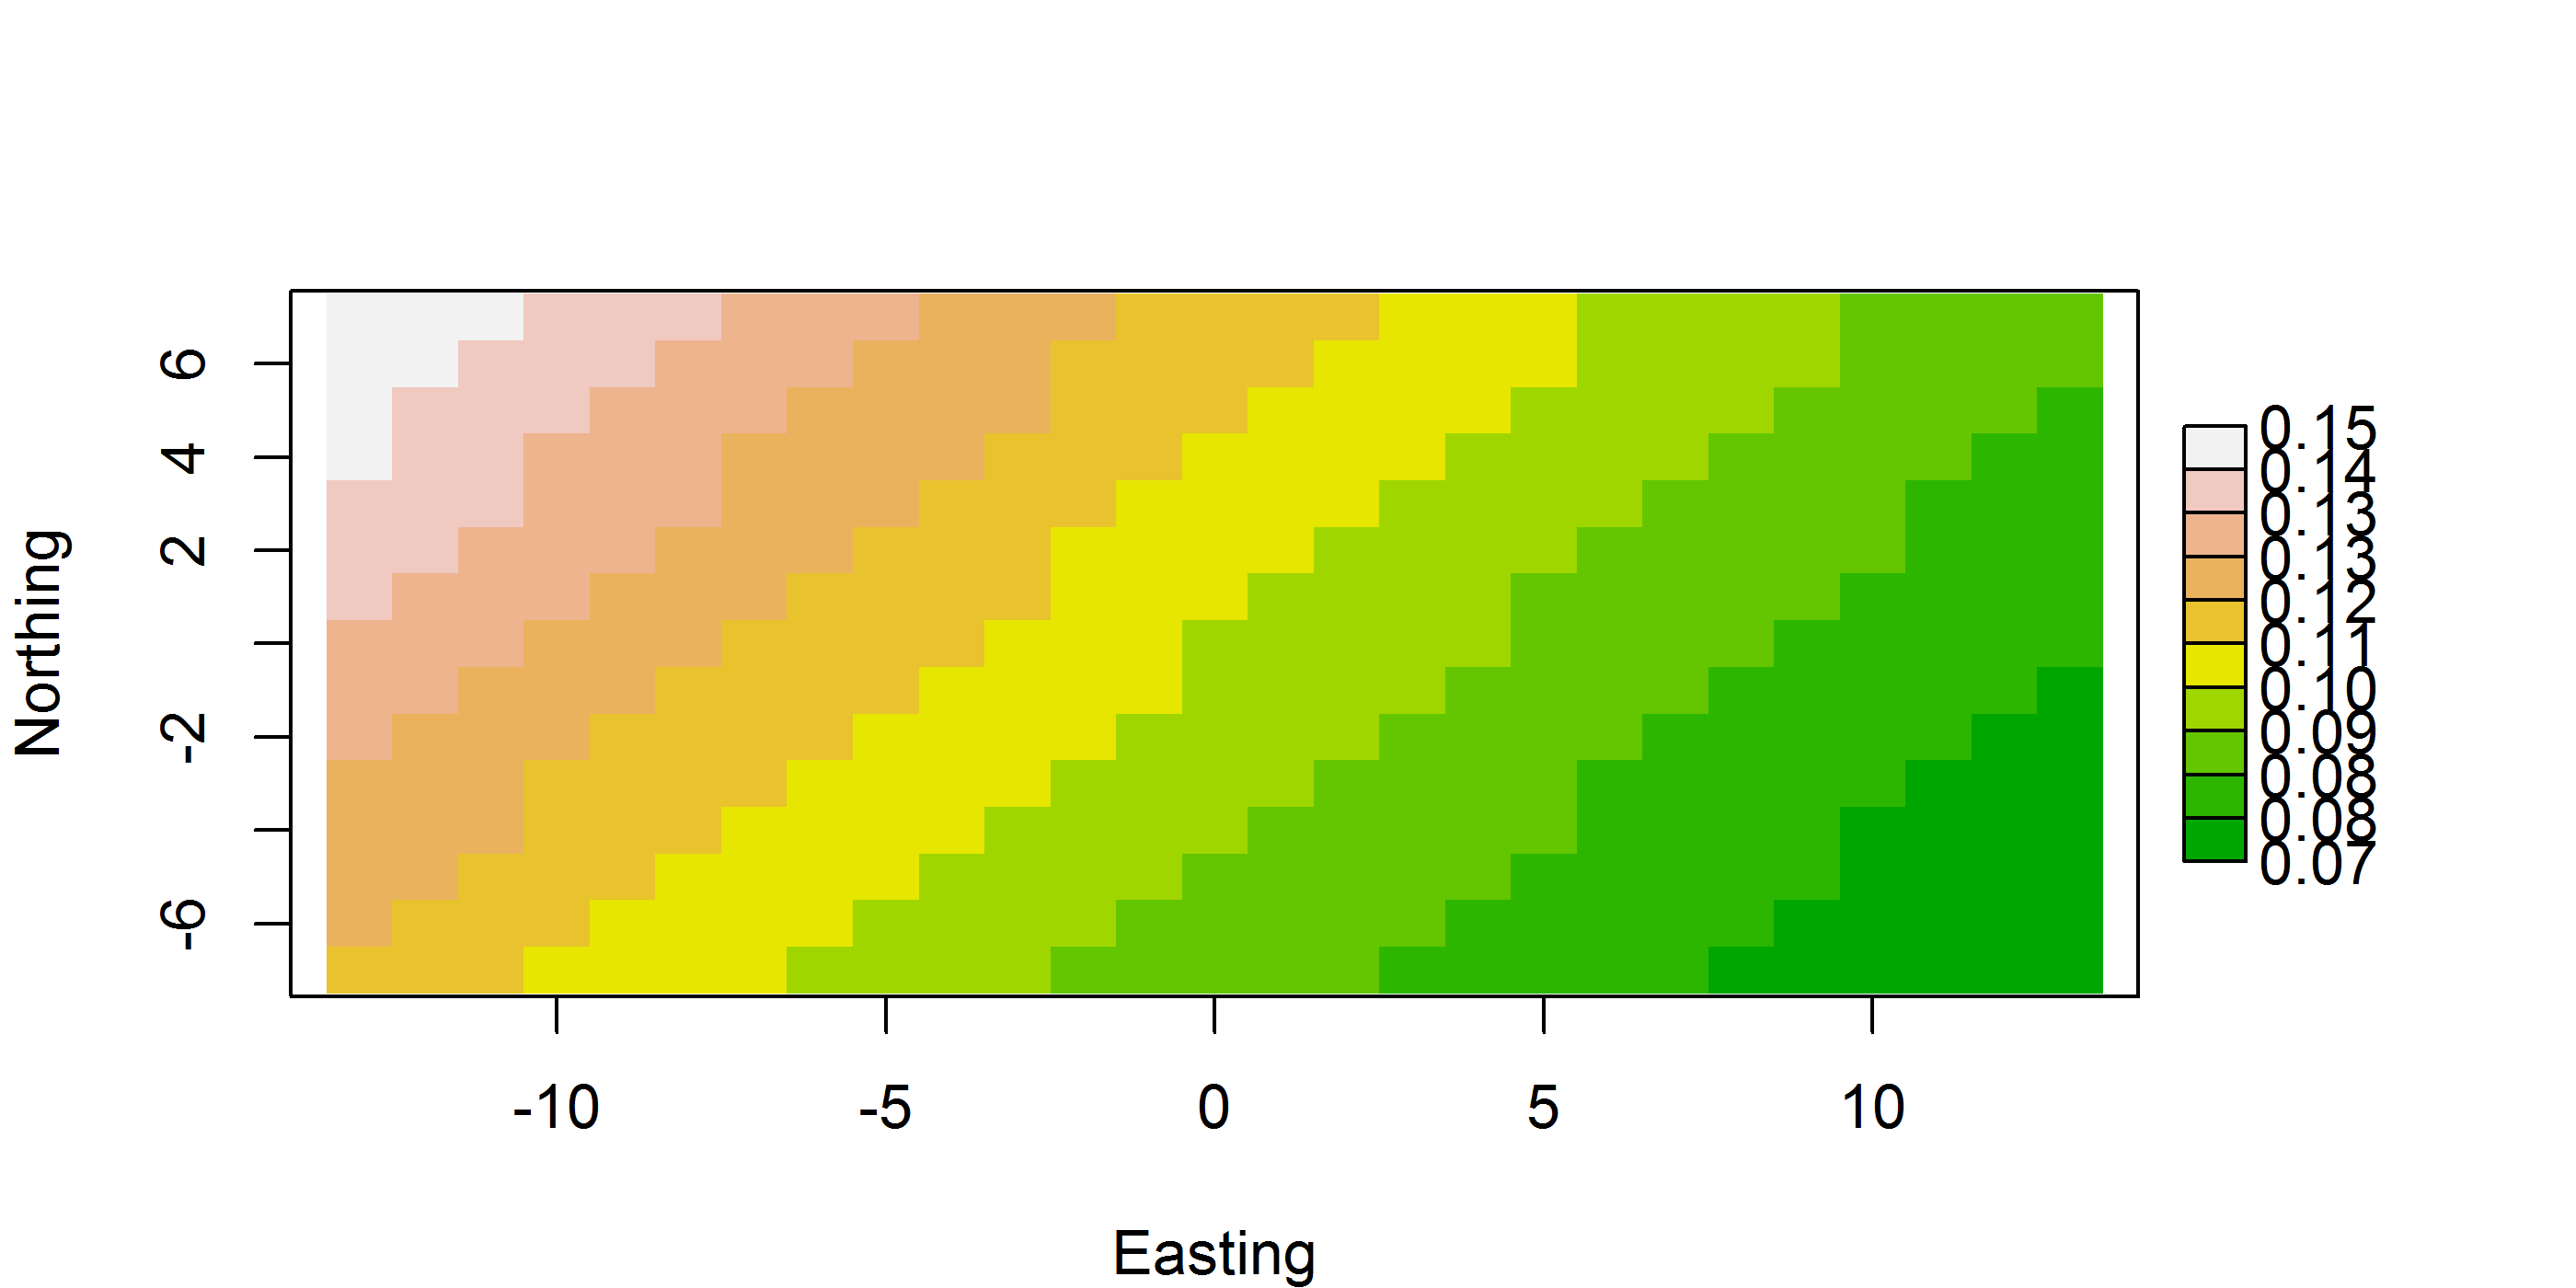
\includegraphics[height=2.5in]{Ch2-Bayes/figs/mallard_gradient}
\end{center}
\caption{Predicted recovery rates of mallard bands in the upper great
  plains of North America. Note the negative gradient from the NW to
  the SE.}
\label{glms.fig.bandrecovery}
\end{figure}

\section{ Summary and Outlook}

GLMs and GLMMs are the most useful statistical methods in all of
ecology. The principles and procedures underlying these methods are
relevant to nearly all modeling and analysis problems in every branch
of ecology. Therefore, understanding how to analyze these models is
an essential skill for the quantitative ecologist to possess.
 If you understand and
can conduct classical likelihood and Bayesian analysis of Poisson and
binomial GLM(M)s, then you will be successful analyzing and
understanding more complex classes of models that arise. We will see
shortly that spatial capture-recapture models are a type of GLMM
and thus having a basic
understanding of the conceptual origins and formulation of GLM(M)s and
their analysis is extremely useful.

We note that GLM(M)s are routinely
analyzed by likelihood methods but we have focused on Bayesian
analysis here in order to develop the tools that are less familiar to
most ecologists, and that we will apply in much of the remainder of the book.  In particular, Bayesian analysis of models with random
effects is relatively straightforward because the models
are easy to analyze conditional on the random effect, using methods of
MCMC.  Thus, we will often analyze SCR models in later chapters by
MCMC, explicitly adopting a Bayesian inference framework.
In that regard, the various {\bf BUGS} engines ({\bf WinBUGS}, {\bf
  OpenBUGS}, {\bf JAGS}; see also \ref{chapt.app1}) are enormously useful because they
provide an accessible platform for
carrying out  analyses by MCMC by just
describing the model, and not having to worry about how to actually
build MCMC algorithms.  That said, the {\bf BUGS} language is more important
than just to the extent that it enables one to do MCMC - it is useful
as a modeling tool because it fosters understanding, in the sense that
it forces you to become intimate with your model. You have to think
about and write
down all of the probability assumptions, and the relationships between
observations and latent variables and parameters in a way that is
ecologically sensible and statistically coherent. Because of this,
that it focuses your thinking on {\it model construction}, 
as M. K\'{e}ry says
in his {\bf WinBUGS} book \citep{kery:2010}, ``{\bf WinBUGS}   frees
the modeler in you.''


While we have emphasized Bayesian analysis in this chapter, and make
primary use of it through the book, we
we will provide an introduction to likelihood analysis in Chapt.
\ref{chapt.mle} and use those  methods also from time to time.
 Before getting to that, however, it will be useful to
talk about more basic, conventional closed population
capture-recapture models and such models are the topic of the next chapter.
